\documentclass[10pt]{beamer}
\usepackage[headerslides]{umnslides}
\usepackage{tikz}
\usepackage{pgfplots}
\usepackage{bm}
\pgfmathsetseed{1234}
\usetikzlibrary{fit,positioning,calc,shapes,backgrounds}
\usetikzlibrary{shapes.geometric, arrows}
\tikzset{>=latex}
\usepackage{tikz-feynman}
\pgfkeys{/tikzfeynman/warn luatex=false}
\usepgfplotslibrary{groupplots}
% \includeonlyframes{current}
\usepackage{listings}

\definecolor{codegreen}{rgb}{0,0.6,0}
\definecolor{codegray}{rgb}{0.5,0.5,0.5}
\definecolor{codepurple}{rgb}{0.58,0,0.82}
\definecolor{backcolour}{rgb}{0.95,0.95,0.92}
\lstdefinestyle{mystyle}{
  backgroundcolor=\color{backcolour},   
  commentstyle=\color{codegreen},
  keywordstyle=\color{magenta},
  numberstyle=\tiny\color{codegray},
  stringstyle=\color{codepurple},
  basicstyle=\ttfamily\footnotesize,
  breakatwhitespace=false,         
  breaklines=true,                 
  captionpos=b,                    
  keepspaces=true,                 
  numbers=left,                    
  numbersep=5pt,                  
  showspaces=false,                
  showstringspaces=false,
  showtabs=false,                  
  tabsize=2
}
\lstset{style=mystyle}




\graphicspath{{./figures}}
\newcommand{\commonfiles}[1]{../common/#1}
\usepackage[mode=buildnew]{standalone}

\author[Charlie Kapsiak (UMN Single Stop Group) ]{
  Nadja Strobbe\inst{1} \and
  Devin Mahon\inst{1} \and
  \underline{Charlie Kapsiak}\inst{1} \and
  Shardul Rao\inst{1} \and
  Seth Bendigo\inst{1}
}


\newif\iflong
\longtrue

\institute{\inst{1}University of Minnesota}

\title[Single Stop Statistics]{RPV Single Stop Search Statistical Inquiry}
\subtitle{Statistical Considerations for Non-parametric 2D Background Estimation Using Gaussian Processes}
\date{2024-09-30}

\begin{document}

\begin{frame}
  \maketitle
\end{frame}

\begin{frame}{Table Of Contents}
  \tableofcontents
\end{frame}

% \iffalse
%   \section{Introduction and Analysis Status}
%   \label{sec:introduction}
%   
%   \begin{frame}{Bump Hunting}
%     \begin{itemize}
%     \item One of the most common classes of searches for new physics are \textit{bump hunts}.
%     \item Given some sort of smooth description of the standard model background, look for a localized bump of excess events coming from a new physics process.
%     \item 
%     \end{itemize}
%     
%     Why bbkg est is important
%   \end{frame}
%   
%   \begin{frame}{Background Estimation Strats}
%     General types of background estimation
%   \end{frame}
%   
%   
%   \begin{frame}{Ad-Hoc}
%     Drawbacks of ad-hoc parametric
%   \end{frame}
%   
%   \begin{frame}{Glimpse of GP}
%     Introduce idea of GP
%   \end{frame}
% \fi

\section[Intro]{Introduction and Analysis Status}

\begin{frame}{Analysis Target}
  \begin{itemize}
  \item Searching for the production and decay of a single \stopq{} to 4 standard model quarks through an RPV coupling. 
  \item Targeting both $\lambda_{312}'',\lambda_{313}'' \in [0.1,0.4]$.
    \begin{itemize}
    \item Intermediate values between long lived ($\lambda < 0.1$) and direct dijet decays ($\lambda > 0.4$)
    \end{itemize}
  \item Well motivated channel to look for SUSY \cite{evans_lhc_2013}:
    \begin{itemize}
    \item Unexplored region of RPV parameter space
    \item Large cross section allows us to probe higher masses
    \end{itemize}
  \item For more information see: %\href{https://indico.cern.ch/event/1324384/\#2-rpv-single-top-squark-analys}{2023-10-06: Introduction Talk}

  \begin{itemize}
    \input{\commonfiles{previous_talks.tex}}
  \end{itemize}
  \end{itemize}

  \begin{center}
    %\graphiccite{figures/xsec.png}{0.5}{rasmussen_gaussian_2006}\hspace{1em}
    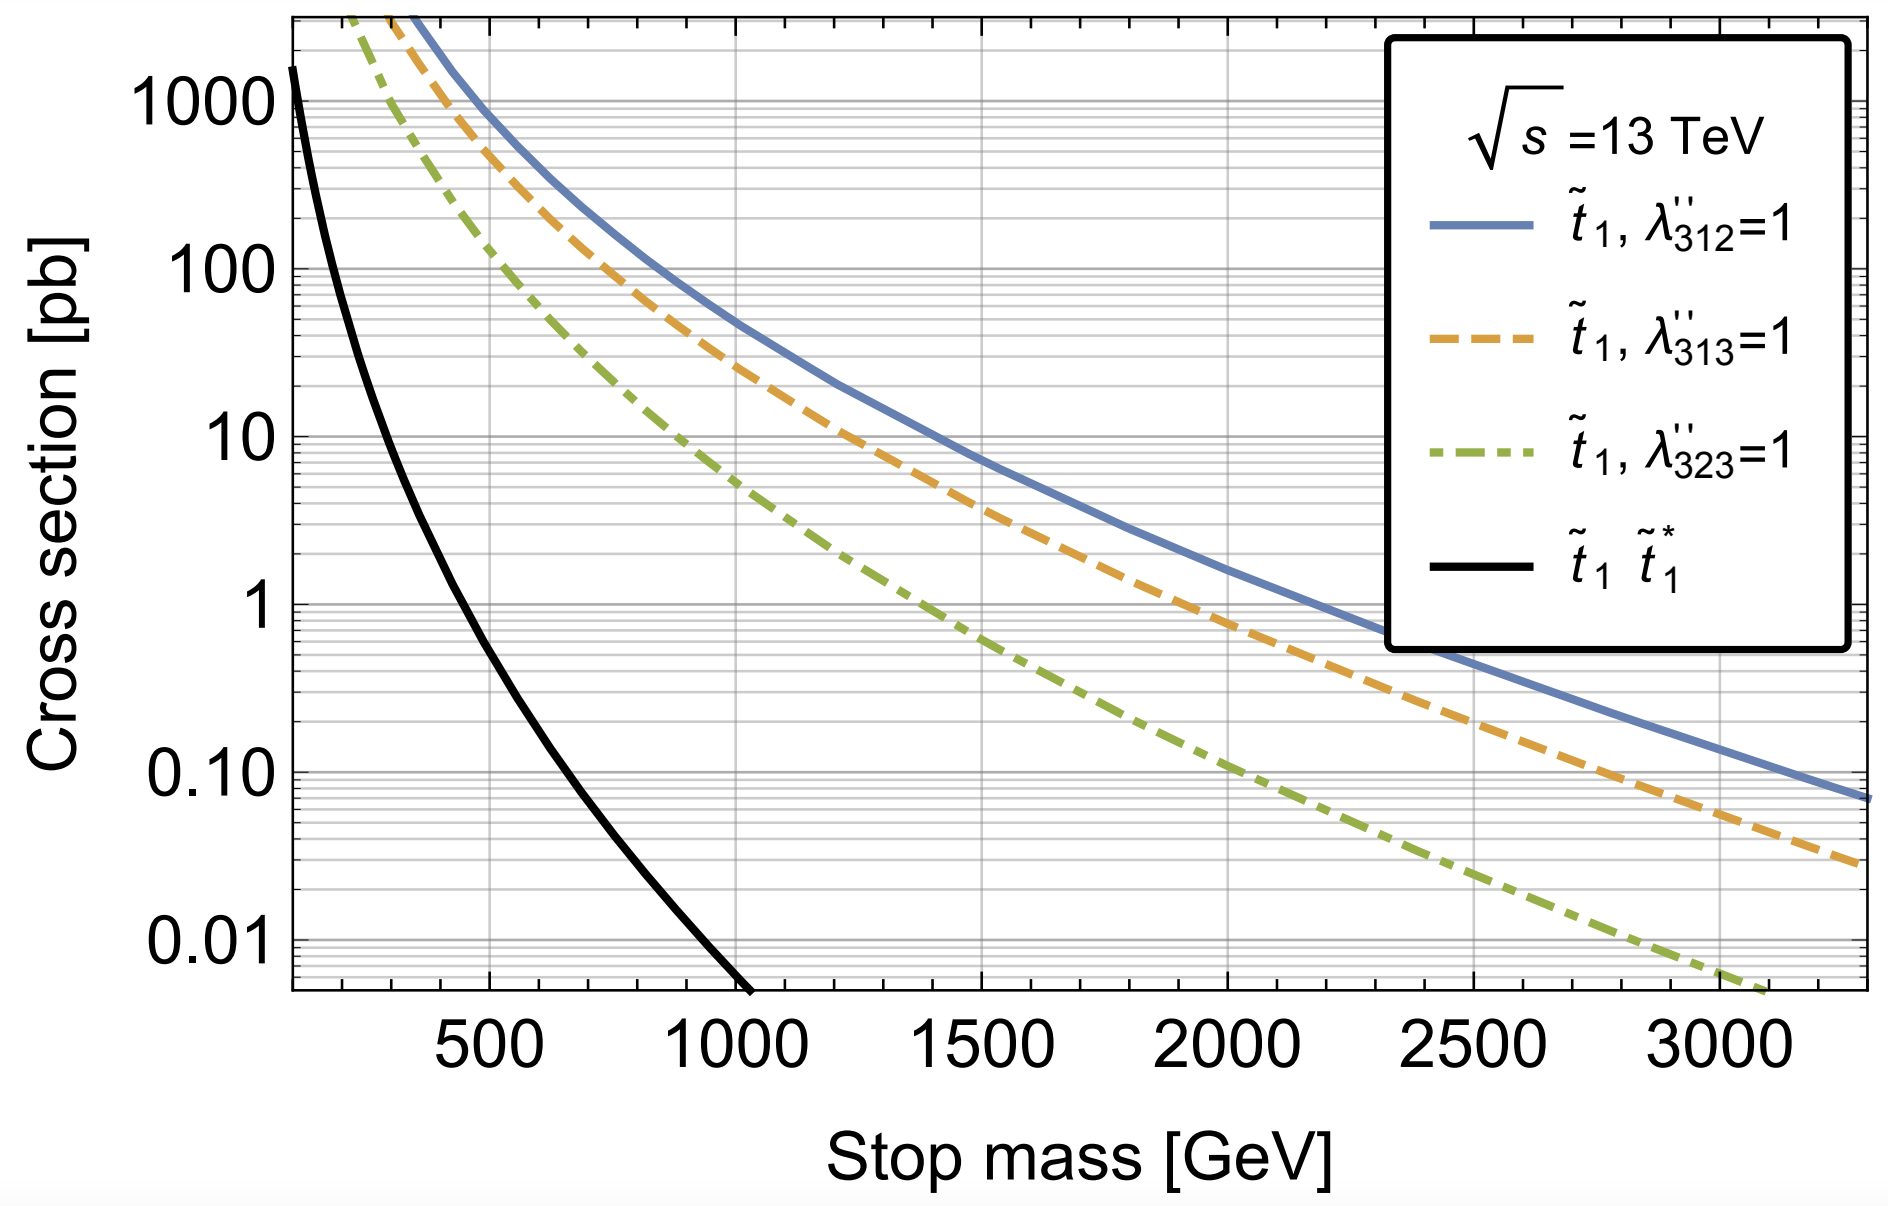
\includegraphics[width=0.5\textwidth]{figures/xsec.png}
    \scalebox{0.7}{\includestandalone{\commonfiles{general/single_stop}}}
  \end{center}

  \begin{beamerpopover}
  \end{beamerpopover}

\end{frame}


% \iflong
%   \begin{frame}{Current Analysis Status}
%     \begin{block}{}
%       The past months have seen substantial progress on several fronts. We summarize below the current major areas of work:
%     \end{block}
%     % \begin{columns}[t]
%     %  \begin{column}{0.5\textwidth}
%     \begin{center} \textbf{Key Analysis Elements} \end{center}
%     \begin{itemize}
%       \coloreditem{ready} Control/Signal region definitions.
%       \coloreditem{working} Mass reconstruction. 
%       \coloreditem{working} Background estimation
%       \coloreditem{prelim} Statistical analysis procedure. 
%       \coloreditem{prelim} Trigger studies.
%       \coloreditem{prelim} Central MC production.
%       \coloreditem{prelim} Early Run3 data.
%     \end{itemize}
%     % \end{column}
%     % \begin{column}{0.5\textwidth}
%     %   \begin{center} \textbf{Past Presentations} \end{center}
%     %   \begin{itemize}
%     %     \input{\commonfiles{previous_talks.tex}}
%     %   \end{itemize}
%     % \end{column}
%     % \end{columns}

%     \begin{center}
%       \begin{tikzpicture}
%         \path[fill=early] (0,0) coordinate (A) circle(0.25em);
%         \node[anchor=left, right=0.1em of A] (A1) {Early Stages} ;

%         \path[fill=prelim] ( $ (A1.east) + (0.2,0)$) coordinate (B) circle(0.25em);
%         \node[anchor=left, right=0.1em of B] (B1) {Preliminary};


%         \path[fill=working] ( $ (B1.east) + (0.2,0) $ ) coordinate (B) circle(0.25em);
%         \node[anchor=left, right=0.1em of B] (C1) {Working Version};

%         \path[fill=ready] ( $(C1.east) + (0.2,0) $) coordinate (D) circle(0.25em);
%         \node[anchor=left, right=0.1em of D] {Analysis Ready};
%       \end{tikzpicture}
%     \end{center}
%   \end{frame}
% \fi



\begin{frame}{Resonance Reconstruction}
  \begin{itemize}
  \item Both the \textcolor{blue}{\stopq{}} and the \textcolor{red}{\chargino{}} form resonances over the background. 
  \item Looking for 2 peaks, $m_{4} \approx m_{\stopq}$ and $m_{3} \approx m_{\chargino}$.
  \item Nearly finalized algorithms for mass recosntruction using a simple NN based jet tagger.
  \item<2-> In two dimensions, resonances can be decorrelated by defining an alternative variable $\frac{m_{3}}{m_{4}}$
  \end{itemize}
  \begin{center}
    \begin{onlyenv}<1>
      \scalebox{0.55}{\includestandalone{\commonfiles{general/two_peaks}}}
    \end{onlyenv}
    \begin{onlyenv}<2->
      \begin{annotimage}{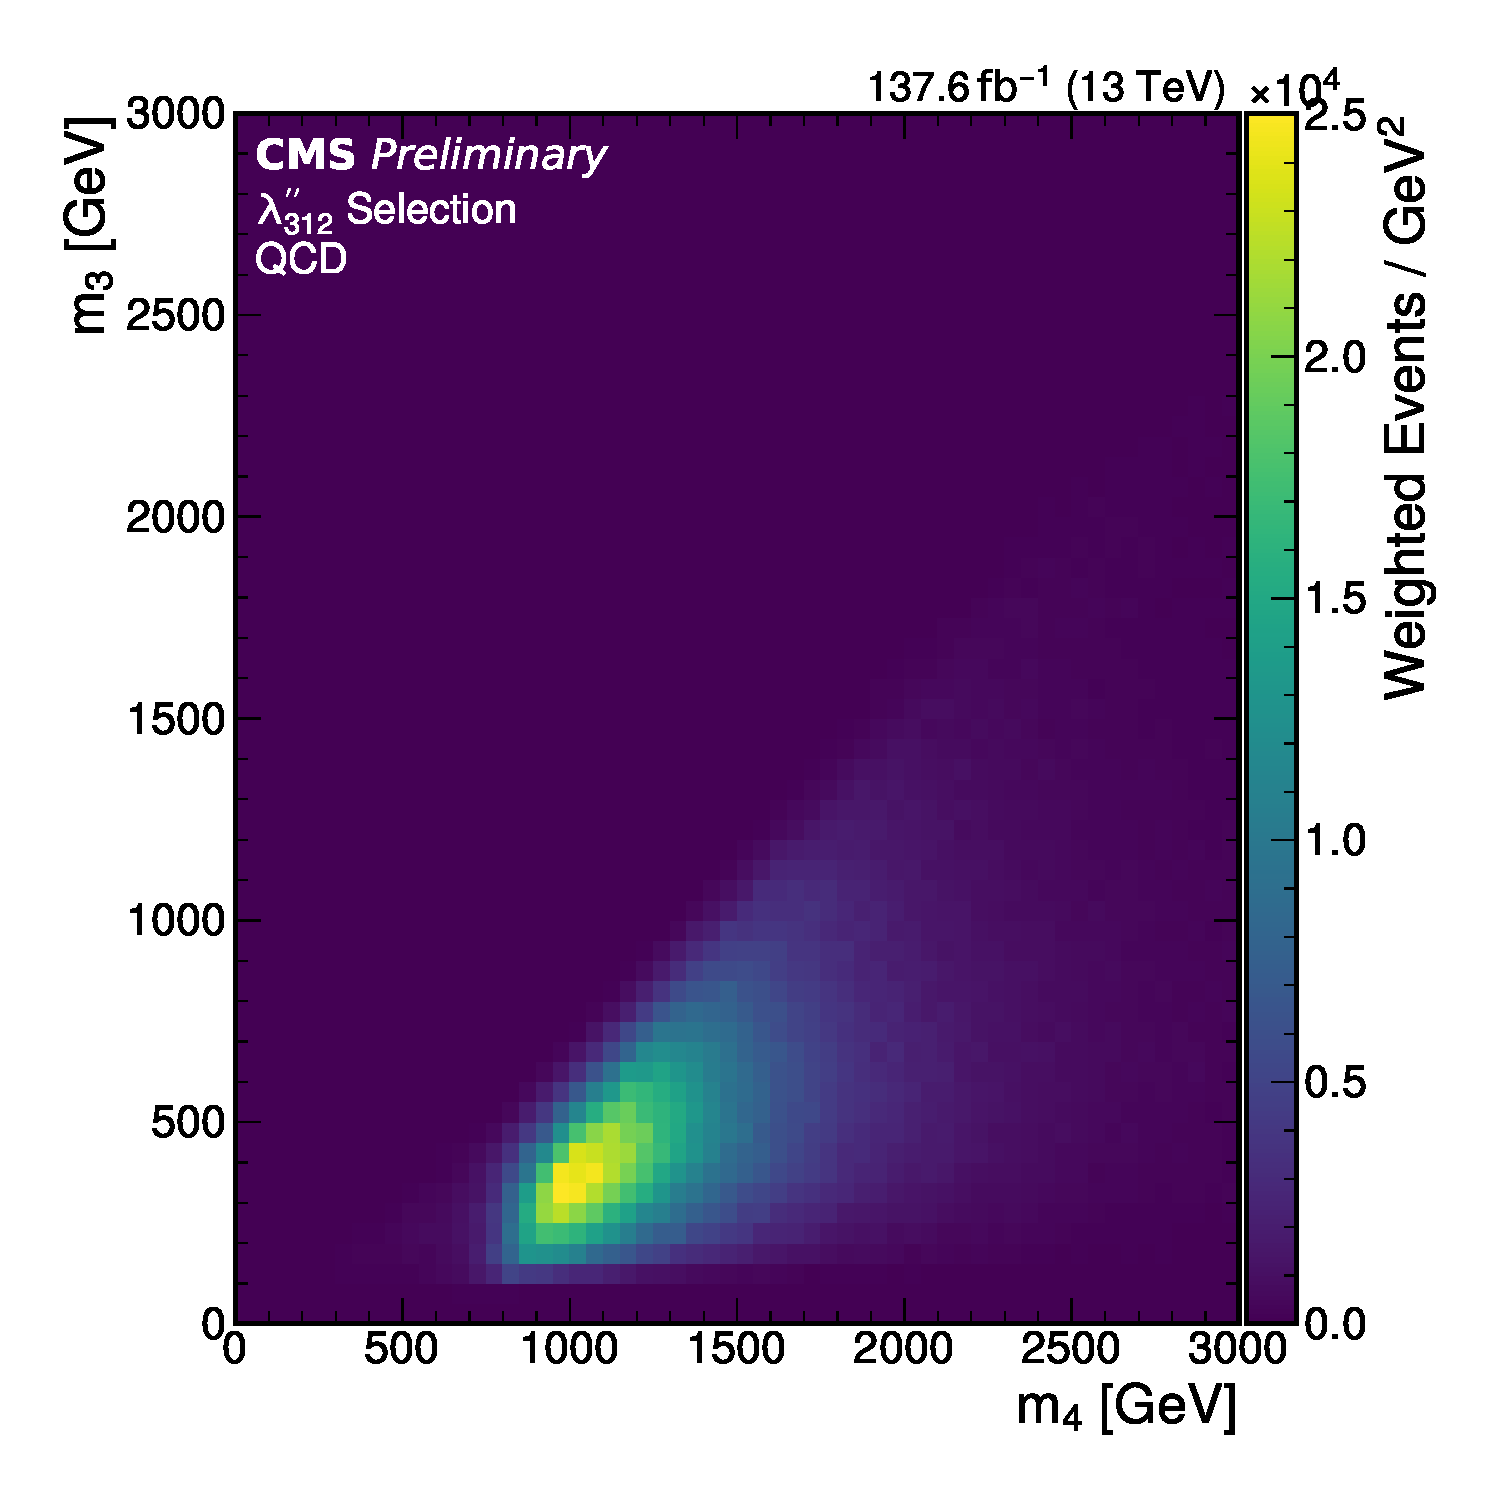
\includegraphics[width=0.30\textwidth]{figures/2d_basic_plots/m14_vs_m24_Skim_QCDInclusive2018.pdf}}
        \node[anchor=south] at (0.5, -0.05){\scriptsize QCD Simulation};
      \end{annotimage}
    \end{onlyenv}
    \begin{onlyenv}<2>
      \begin{annotimage}{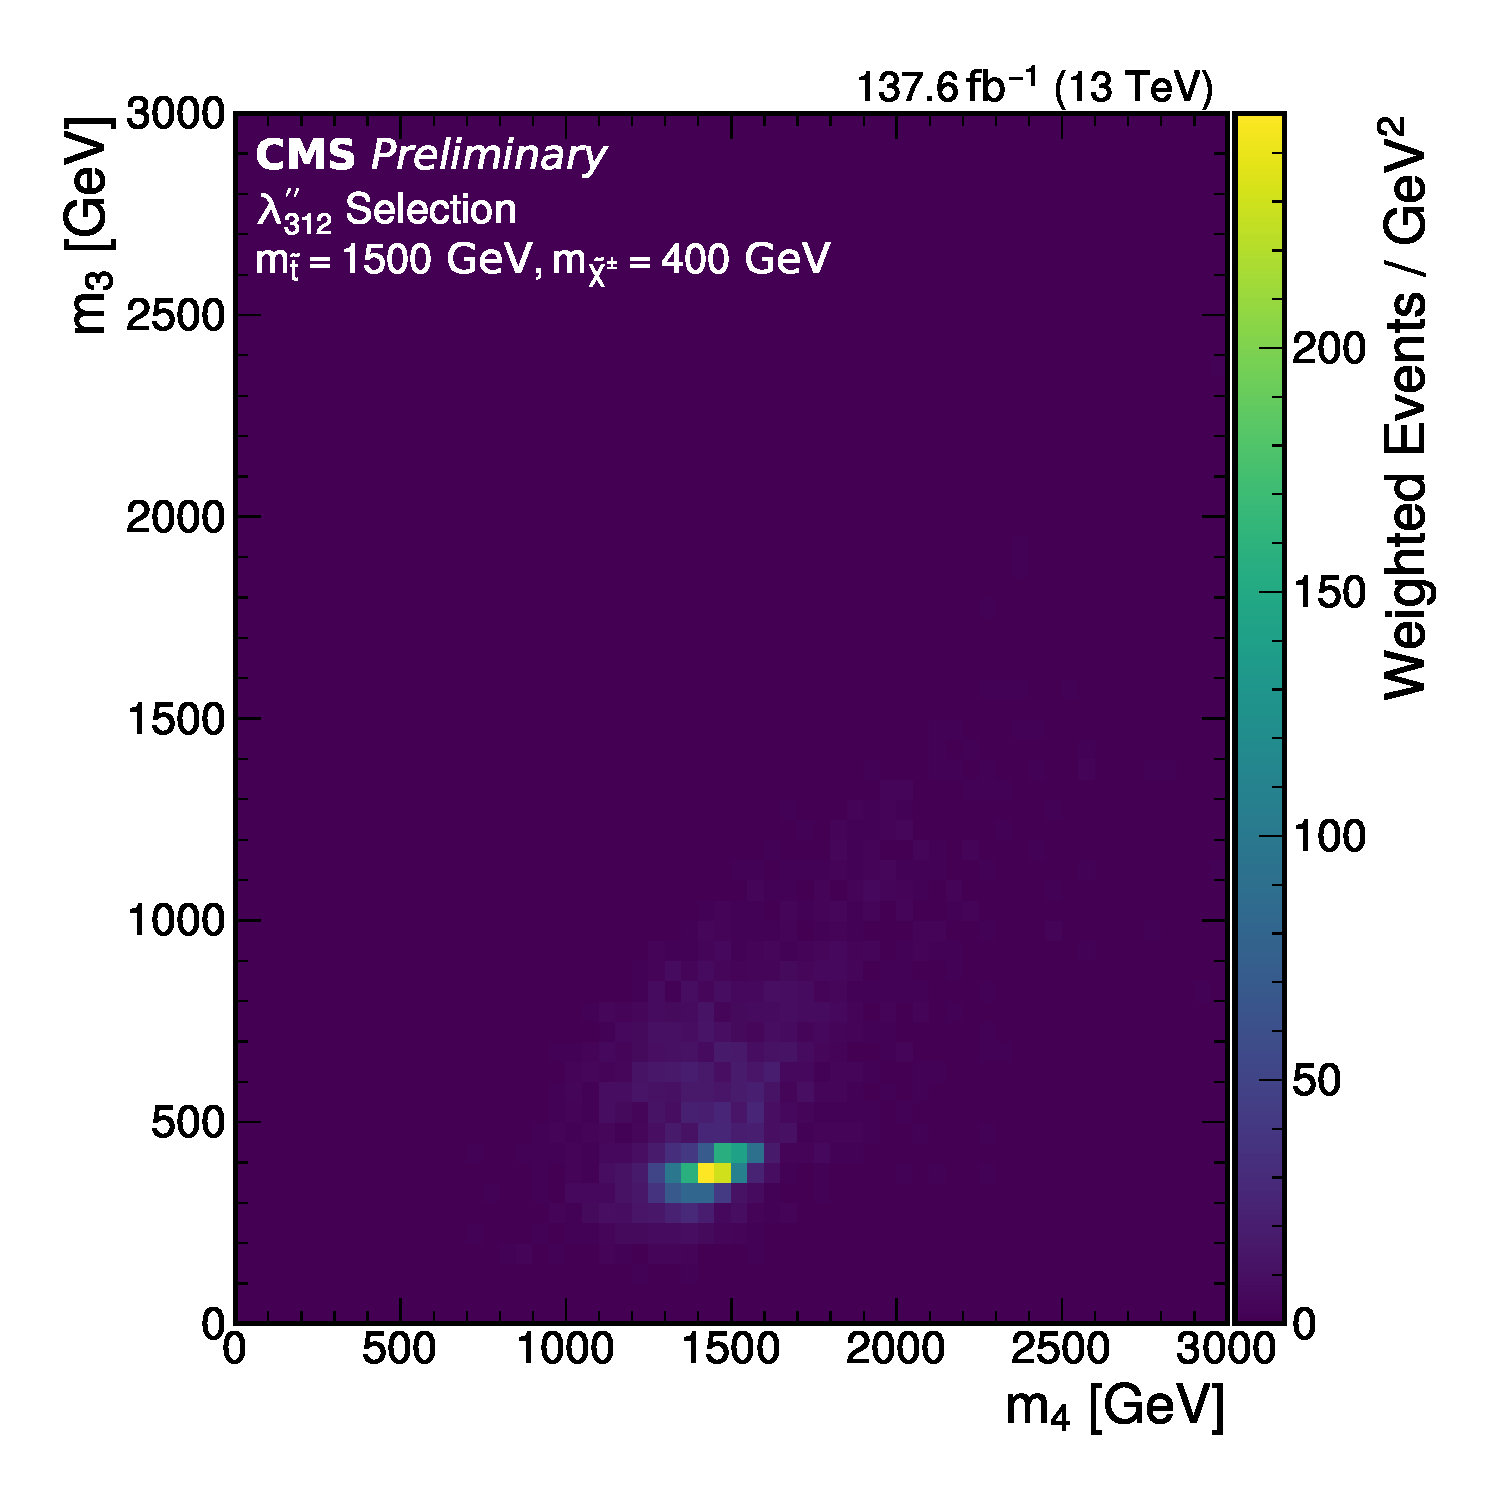
\includegraphics[width=0.30\textwidth]{figures/2d_basic_plots/m14_vs_m24_signal_312_1500_400.pdf}}
        \node[anchor=south] at (0.5, -0.05){\scriptsize Signal};
      \end{annotimage}
    \end{onlyenv}
    \begin{onlyenv}<3>
      \begin{annotimage}{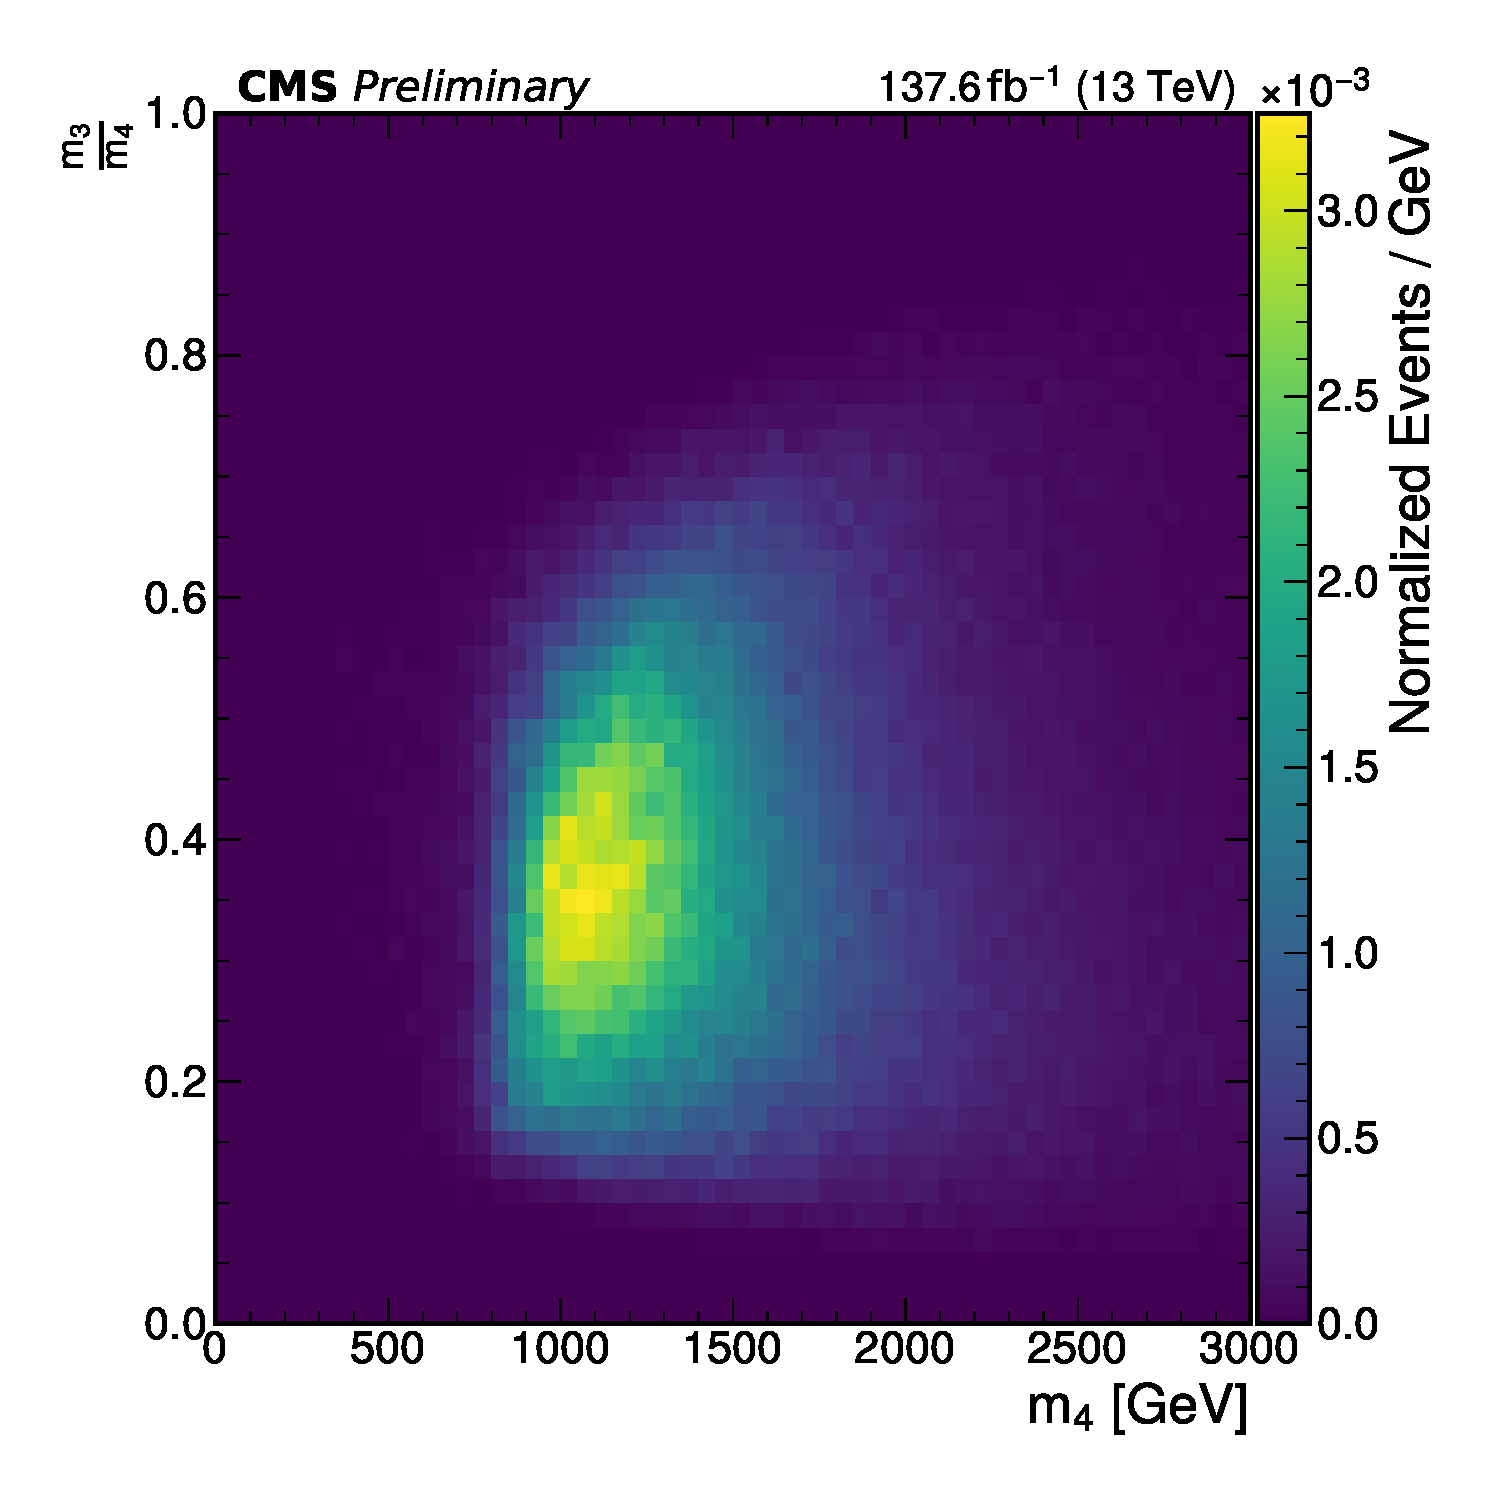
\includegraphics[width=0.30\textwidth]{figures/2d_basic_plots/ratio_m14_vs_m24_Skim_QCDInclusive2018.pdf}}
        \node[anchor=south] at (0.5, -0.05){\scriptsize QCD Simulation Decorrelated};
      \end{annotimage}
      \begin{annotimage}{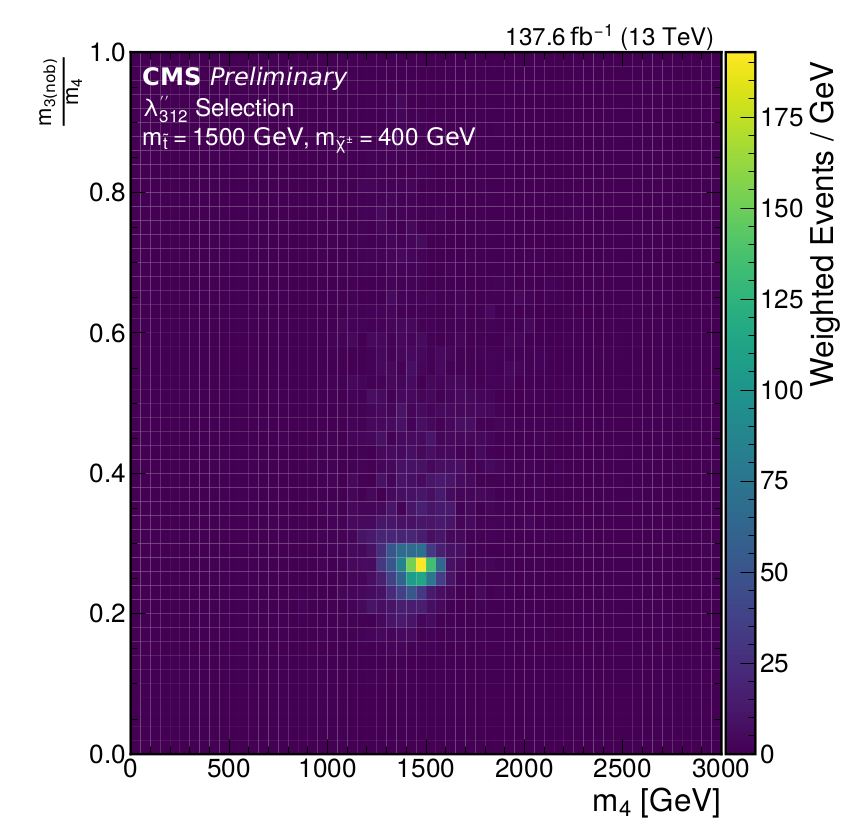
\includegraphics[width=0.30\textwidth]{figures/2D_peak}}
        \node[anchor=south] at (0.5, -0.05){\scriptsize Signal Decorr};
      \end{annotimage}
    \end{onlyenv}
  \end{center}
\end{frame}

\begin{frame}{General Search Strategy}
  \begin{itemize}
  \item General search strategy is to perform a one or two dimensional bump hunt for both the \textcolor{blue}{\stopq{}} and the \textcolor{red}{\chargino{}} resonances. 
  \item For many mass splittings, the resonances are well separated both in \textcolor{blue}{$m_{\stopq, reco}$} and \textcolor{red}{$m_{\chargino, reco}$} space, providing additional discriminating power.
  \item Key point is to effectively estimate the background. 
  \item However, a simple cut strategy on one mass axis can result in sculpting of the background, making estimation difficult. We must therefore model correlations appropriately, or seek a method that handles this automatically.
  \end{itemize}
  \vspace{-0.5cm}
  \begin{tikzpicture}
  \end{tikzpicture}
  \begin{center}
    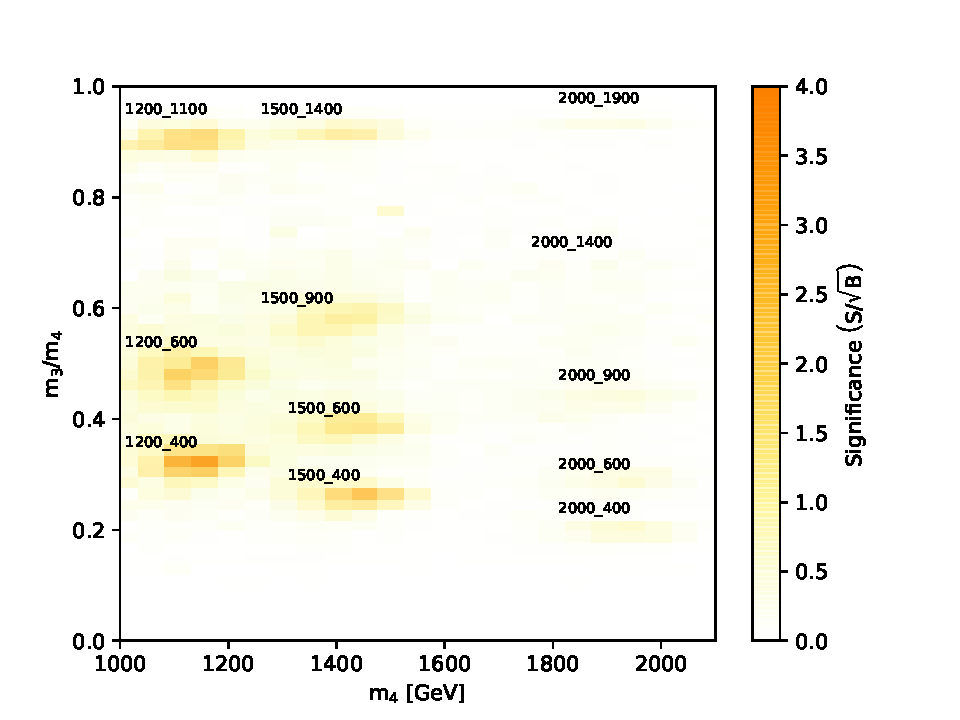
\includegraphics[width=0.4\textwidth]{figures/SigPlotLPPFactor1.pdf}
    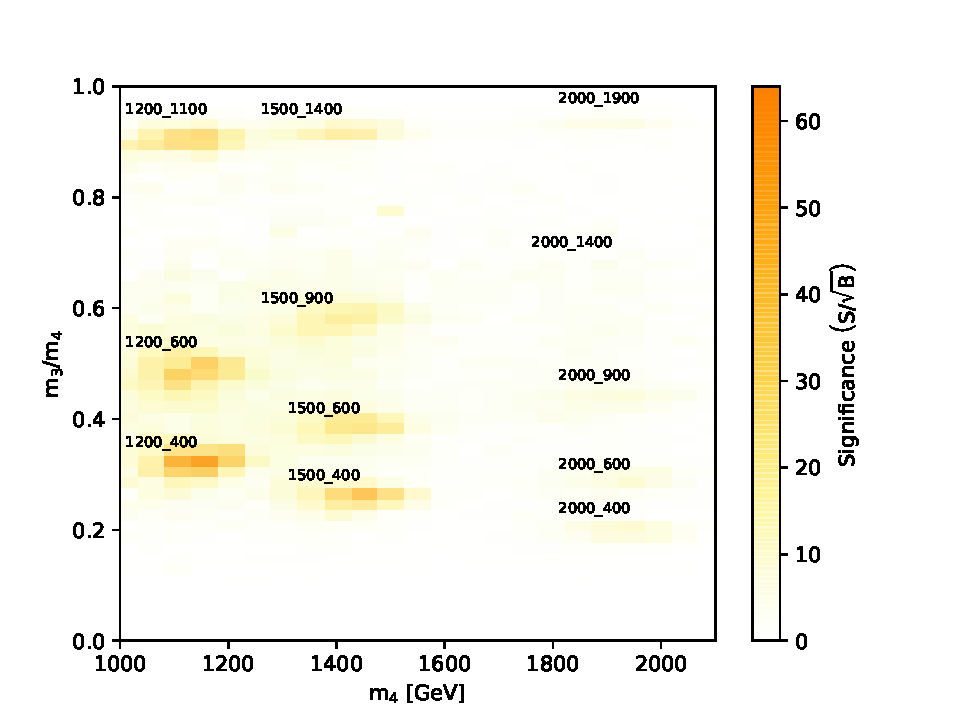
\includegraphics[width=0.4\textwidth]{figures/SigPlotLPPFactor16.pdf}
    % \scalebox{0.5}{\includestandalone{\commonfiles{general/two_peaks}}}\hspace{1cm}
    % 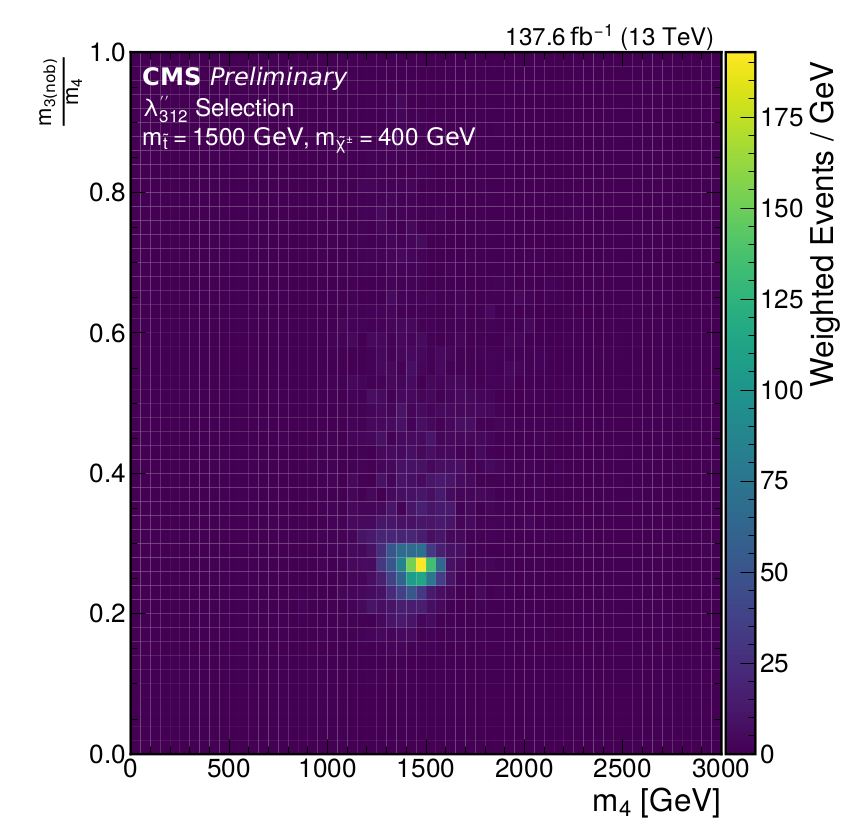
\includegraphics[width=0.35\textwidth]{figures/2D_peak}
  \end{center}
  \begin{center}
    \tiny Plots showing the simple significance $\text{S} / \sqrt{\text{B}}$ for $\lambda_{312}''=0.1$(left) and $\lambda_{312}''=0.4$ (right).
  \end{center}
\end{frame}


% \begin{frame}{Estimation Strategies}
%   \begin{splitcol}[0.55]
%     \begin{col}
%       \begin{itemize}
%       \item For all bump hunts, key technique is estimation of the background shape.
%         The region where signal is expected is blinded, then the fit is used to estimated the background.
%       \item Traditional bump hunts have used ad-hoc functions \cite{zisopoulos_parametric_2023}, chosen because they approximate the observed shape. 
%       \item However, this can introduce bias from the choice of function, and it has been shown that they scale poorly with increasing luminosity \cite{frate_modeling_2017}.
%       \item For multidimensional searches, the problem can also be compounded by the complexity of selecting an appropriate 2D function.
%       \end{itemize}
%     \end{col}
%     \begin{col}
%       \begin{center}
%         \begin{onlyenv}<1>
%           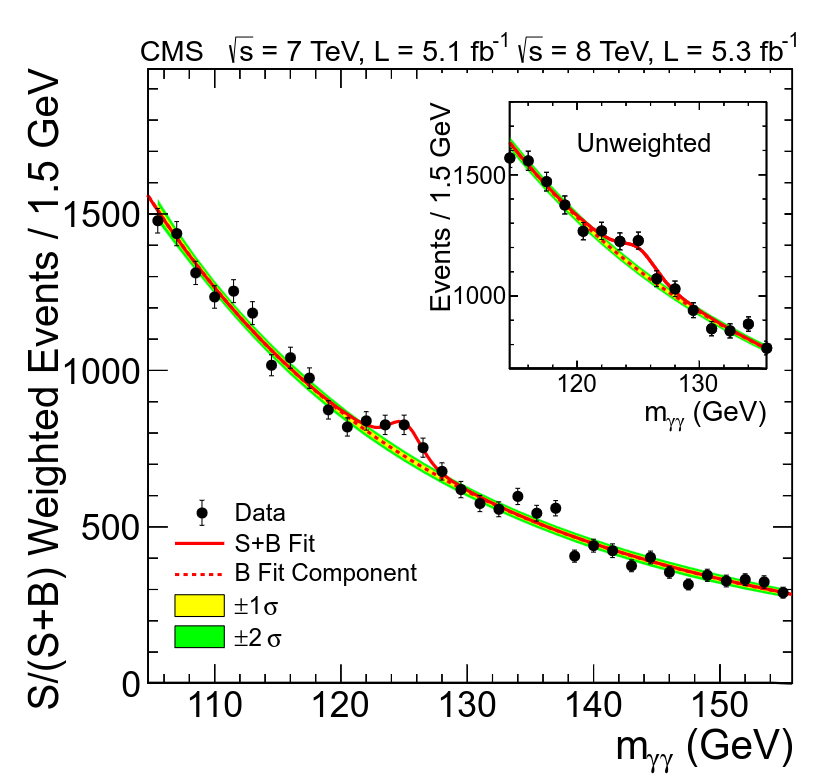
\includegraphics[width=\textwidth]{figures/higgs}
%         \end{onlyenv}
%         \begin{onlyenv}<2>
%           \graphiccite{figures/fit_table}{1}{zisopoulos_parametric_2023}
%         \end{onlyenv}
%       \end{center}
%     \end{col}
%   \end{splitcol}
% \end{frame}

\begin{frame}{Current Strategy}
  \begin{itemize}
  \item We have implemented our background estimation using Gaussian process regression (GPR) \cite{rasmussen_gaussian_2006}.
  \item It has been shown to be robust against increasing luminosity\cite{frate_modeling_2017}.
  \item It is naturally extensible to multiple dimensions.
  \item Very well studied in statistics literature\cite{rasmussen_gaussian_2006}, and has a large number of well established implementations \cite{noauthor_comparison_2024, gardner_gpytorch_2021}.
  \item 1D GPR been used in approved analysis EXO-21-004 \cite{cms_collaboration_searches_2024}.
  \end{itemize}
\end{frame}

% \section[Gaussian Process Regression]{Gaussian Process Regression Overview}
% \label{sec:gauss-proc-regr}


% \begin{frame}{Representing Histograms With Gaussians}
%   \begin{overprint}
%     \begin{itemize}
%     \item We seek a way to describe our histogram probabilistically without reference to a specific parametric form. How can this be done?
%     \item The answer: consider each of the N bins to be a random variable: part of a Multivariate Normal (MVN).
%     \item<1-> Consider our falling mass distribution.
%     \item<2-> Imagine for simplicity we rebinned to have just 2 bins.
%     \item<3-> We can represent the underlying distribution as a 2D Gaussian.
%     \end{itemize}
%   \end{overprint}
%   \begin{overprint}
%     \begin{center}
%       \begin{onlyenv}<1>
%         \scalebox{0.5}{\includestandalone{\commonfiles{gp/histogram}}}
%       \end{onlyenv}
%     \end{center}
%     \def\meanOne{0.8}
%     \def\meanTwo{0.4}
%     \def\binOne{0.7}
%     \def\binOneStd{0.1}
%     \def\binTwo{0.48}
%     \def\binTwoStd{0.1}

%     \begin{onlyenv}<2> %
%       \begin{center}
%         \scalebox{0.5}{\includestandalone{\commonfiles{gp/sampled_hist}}}%
%       \end{center}
%     \end{onlyenv}

%     \begin{onlyenv}<3>
%       \begin{center}
%         \scalebox{0.5}{\includestandalone{\commonfiles{gp/independent}}}%
%         \scalebox{0.5}{\includestandalone{\commonfiles{gp/sampled_hist}}}%
%       \end{center}
%     \end{onlyenv}%
%     \foreach \one/\two [count=\n] in {\meanOne/\meanTwo, 0.6/0.2, 0.9/0.1} { %
%       \pgfmathtruncatemacro\z{\n+3} %
%       \only<\z>{ %
%         \def\binOne{\one} %
%         \def\binTwo{\two} %
%         \begin{center}
%           \scalebox{0.5}{\includestandalone{\commonfiles{gp/sampled_2d}}} %
%           \scalebox{0.5}{\includestandalone{\commonfiles{gp/sampled_hist}}}
%         \end{center}
%       } %
%     }
%   \end{overprint}
% \end{frame}

% \begin{frame}{Prediction}
%   \begin{itemize}
%   \item The previous slide shows how we can use an MVN to describe a histogram.
%   \item How can we have actual predictive power? How can we incorporate known data to extrapolate to unknown points?
%   \item Answer: Condition the gaussian! If $p(b_{1},b_{2}) \sim \mathcal{N}(b_{1},b_{2})$ then $p(b_{1} | b_{2,obs} ) \sim  \mathcal{N}(b_{1},b_{2,obs})$
%   \end{itemize}
%   \begin{center}
%     \def\meanOne{0.8}
%     \def\meanTwo{0.4}
%     \def\binOne{0.7}
%     \def\binTwo{0.48}
%     \def\binTwoStd{0.1}
%     \scalebox{0.5}{\includestandalone{\commonfiles{gp/conditioned_2d}}} %
%     \scalebox{0.5}{\includestandalone{\commonfiles{gp/conditioned_hist}}} %
%   \end{center}
  
% \end{frame}


% \begin{frame}{Beyond the Histogram}
%   \begin{itemize}
%   \item What if we have more than 2 bins? What if we have infinitely many bins (ie a function)?
%   \item How should we describe the MVN then?
%   \end{itemize}
% \end{frame}

% \begin{frame}{What is a Gaussian Process?}
%   \begin{definition}
%     A gaussian process is a possibly infinite series of random variables, any finite subset of which is jointly gaussian.
%   \end{definition}
%   Generally, the random variables are indexed by real values $x$, since we are generally considering regression over $\mathbb{R}^{n}$.

%   A gaussian process $f(x)$ is completely defined by its mean and covariance
%   \begin{equation}
%     \begin{split}
%       \markpos{gpmean}{m(x)} &= \mathbb{E} \left[ f(x) \right] \\
%       \markpos{gpk}{k(x,x')} &= \mathbb{E} \left[ \left( f(x) - m(x) \right)  \left( f(x') - m(x') \right)\right] 
%     \end{split}
%   \end{equation}

%   \begin{center}
%     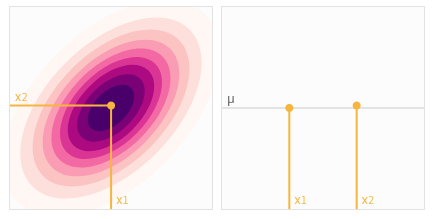
\includegraphics[width=0.4\textwidth]{figures/two_points_1}
%     \hspace{1cm}
%     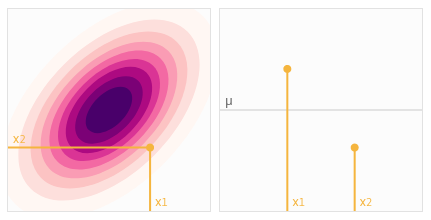
\includegraphics[width=0.4\textwidth]{figures/two_points_2}
%   \end{center}

%   \begin{onlyenv}<2>
%     \posannot[20:3cm]{gpmean}{fill=UMNMaroon!10, draw=UMNMaroon}{The mean value of the MVN == Background Estimate }
%     \posannot[-30:4cm]{gpk}{fill=UMNMaroon!10, draw=UMNMaroon}{The covariance between  any two points. \\ These are the background estimate error bars.}
%   \end{onlyenv}
% \end{frame}

% % \begin{frame}{Gaussian Process Regression}
% %   \begin{itemize}
% %   \item The ability to define distributions over functions allows us to do inference using Baye's theorem. 
% %   \item Specifically, given $N$ training points and a Gaussian process prior, we can produce a posterior Gaussian process that provides a means to do regression. 
% %   \end{itemize}
% %   \begin{center}
% %     \graphiccite{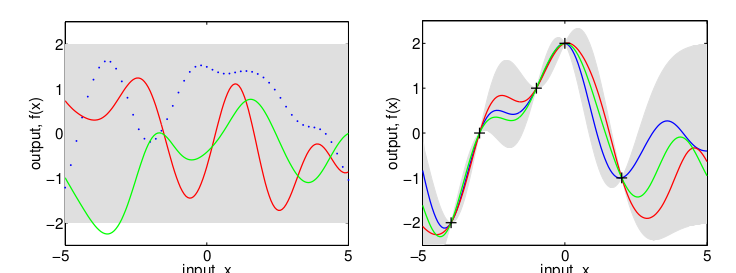
\includegraphics[width=0.7\textwidth]{figures/prior_and_conditioning}}{\cite{rasmussen_gaussian_2006}}
% %   \end{center}
% % \end{frame}

% \begin{frame}[label=kernelscales]{Kernels and Scales}
%   \begin{itemize}
%   \item The choice of kernel is the most important aspect of Gaussian processes. 
%   \item The choice of $k(x,y)$ reflects our understanding of how the points should be correlated, how smooth the functions should be, etc. 
%   \item The choice of kernel consists of both the selection of the form and the hyperparameters. 
%   \item The form of the kernel is chosen to reflect prior understanding of how regions of space should be related.
%   \item One a kernel is chosen, hyperparameters are determined algorithmically, so as to maximize the marginal log likelihood: 
%   \end{itemize}
%   \begin{equation}
%     \log p(\bm{y}|X) =
%     \markpos{term1}{-\frac{1}{2}\bm{y}^T(K+\sigma^2_n I)^{-1}\bm{y}}
%     - \markpos{term2}{\frac{1}{2}\log|K+\sigma^2_n I|}
%     - \frac{n}{2}\log2\pi
%   \end{equation}
%   \begin{onlyenv}<2>
%     \posannot{term1}{fill=UMNMaroon!10, draw=UMNMaroon}{Compatibility of model with data}
%     \posannot[210:3cm]{term2}{fill=UMNMaroon!10, draw=UMNMaroon}{Overfitting penalty works against kernels with large determinants.}
%   \end{onlyenv}
% \end{frame}

% \begin{frame}{Kernels and Scales Continued}
%   \begin{itemize}
%   \item The most common kernel is the RBF kernel
%     \begin{equation}
%       k_{\text{RBF}}(\mathbf{x_1}, \mathbf{x_2}) = \exp \left( -\frac{1}{2} \frac{(\mathbf{x_1} - \mathbf{x_2})^2}{ \ell^{2}} \right)
%     \end{equation}
%   \item Let us see how this kernel lets us extrapolate $m_{\stopq}$ in to the blinded window indicated by the red bars, for different length scales $\ell$, using QCD Simulation on $m_{\stopq}$.
%   \end{itemize}

%   \begin{center}
%     \blockcite{\markimage{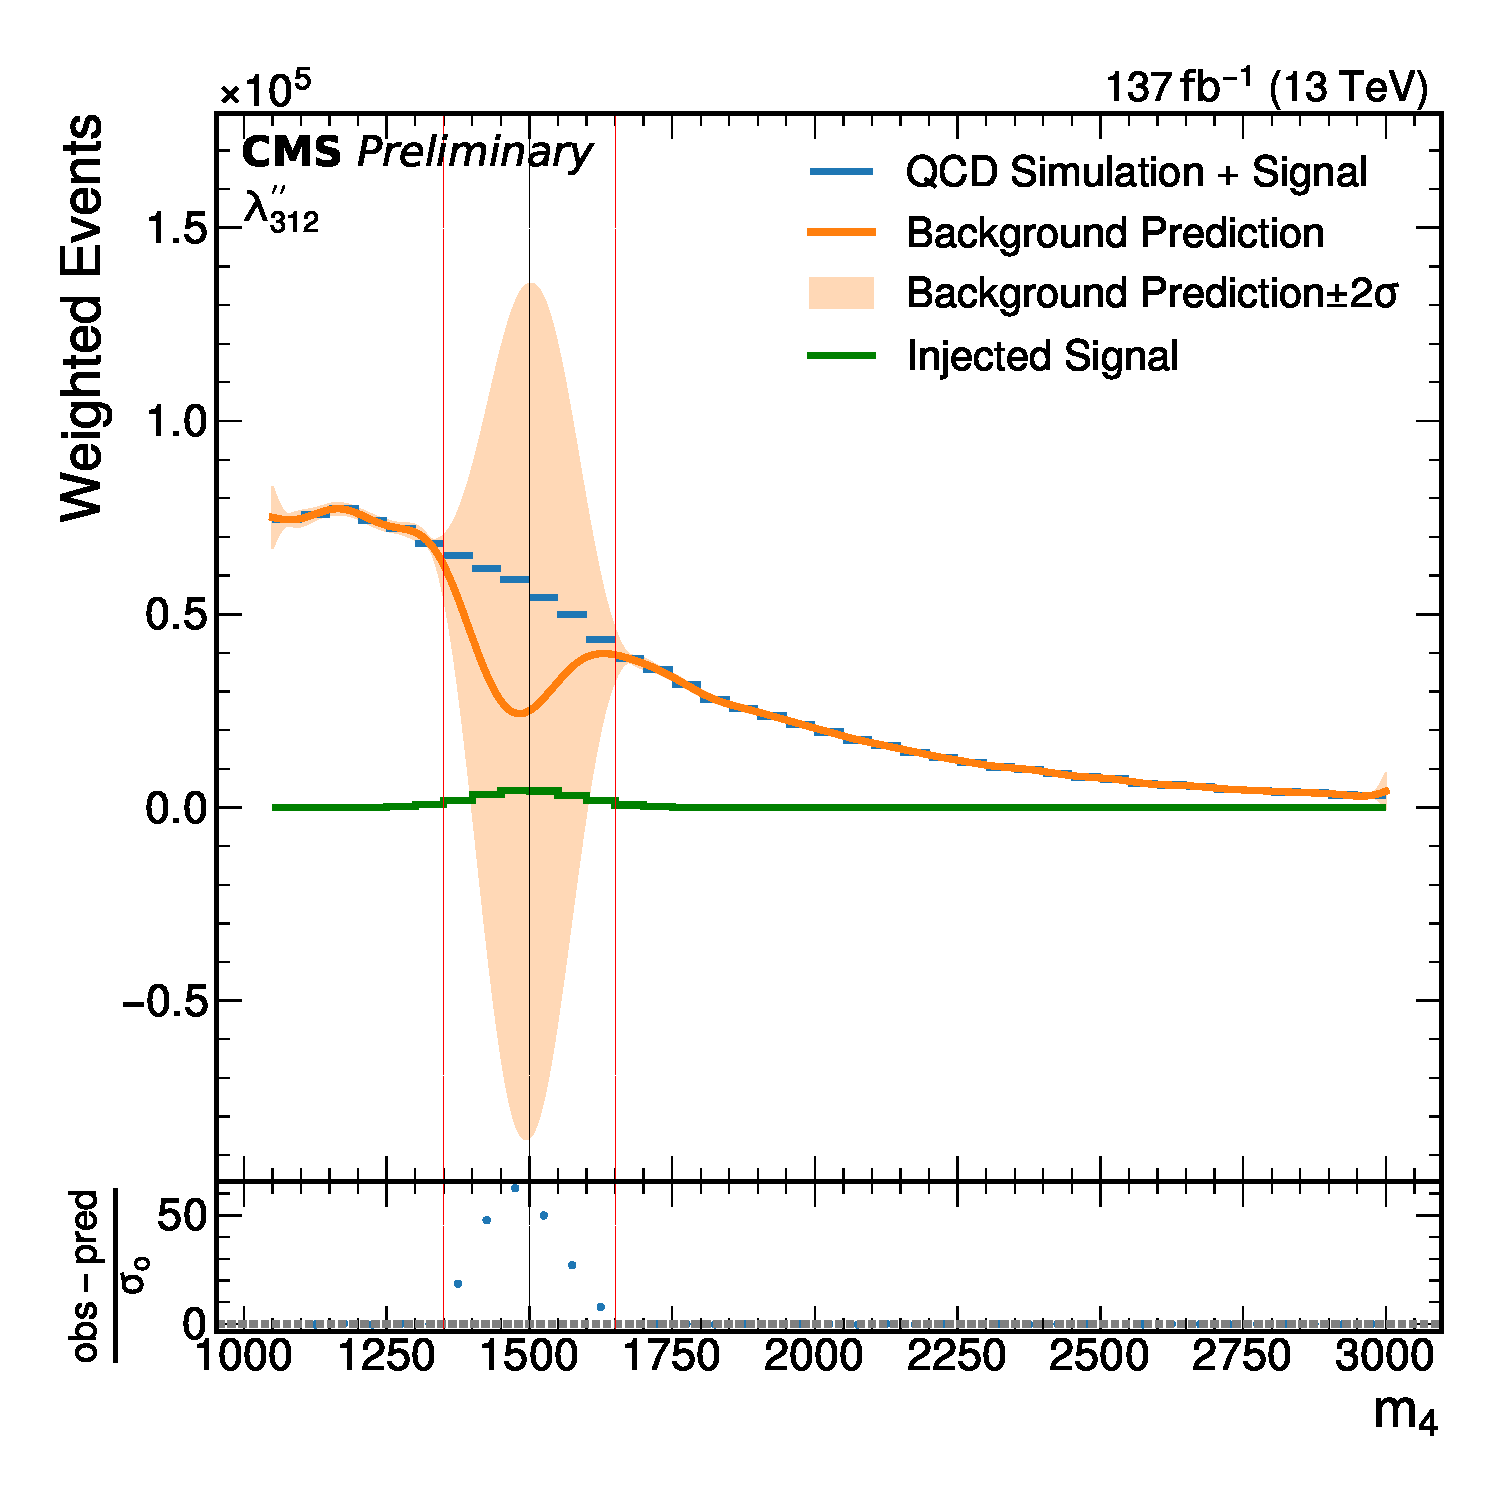
\includegraphics[width=0.31\textwidth]{figures/fitplots/pull_sr_inj_signal_312_1500_1400__lb1050__r15p0__fs_100p0__m1500p0_s90p0__w_1350p0_1650p0}}{0.4,0.6}{ls1}}{Scale = 100GeV}
%     \blockcite{{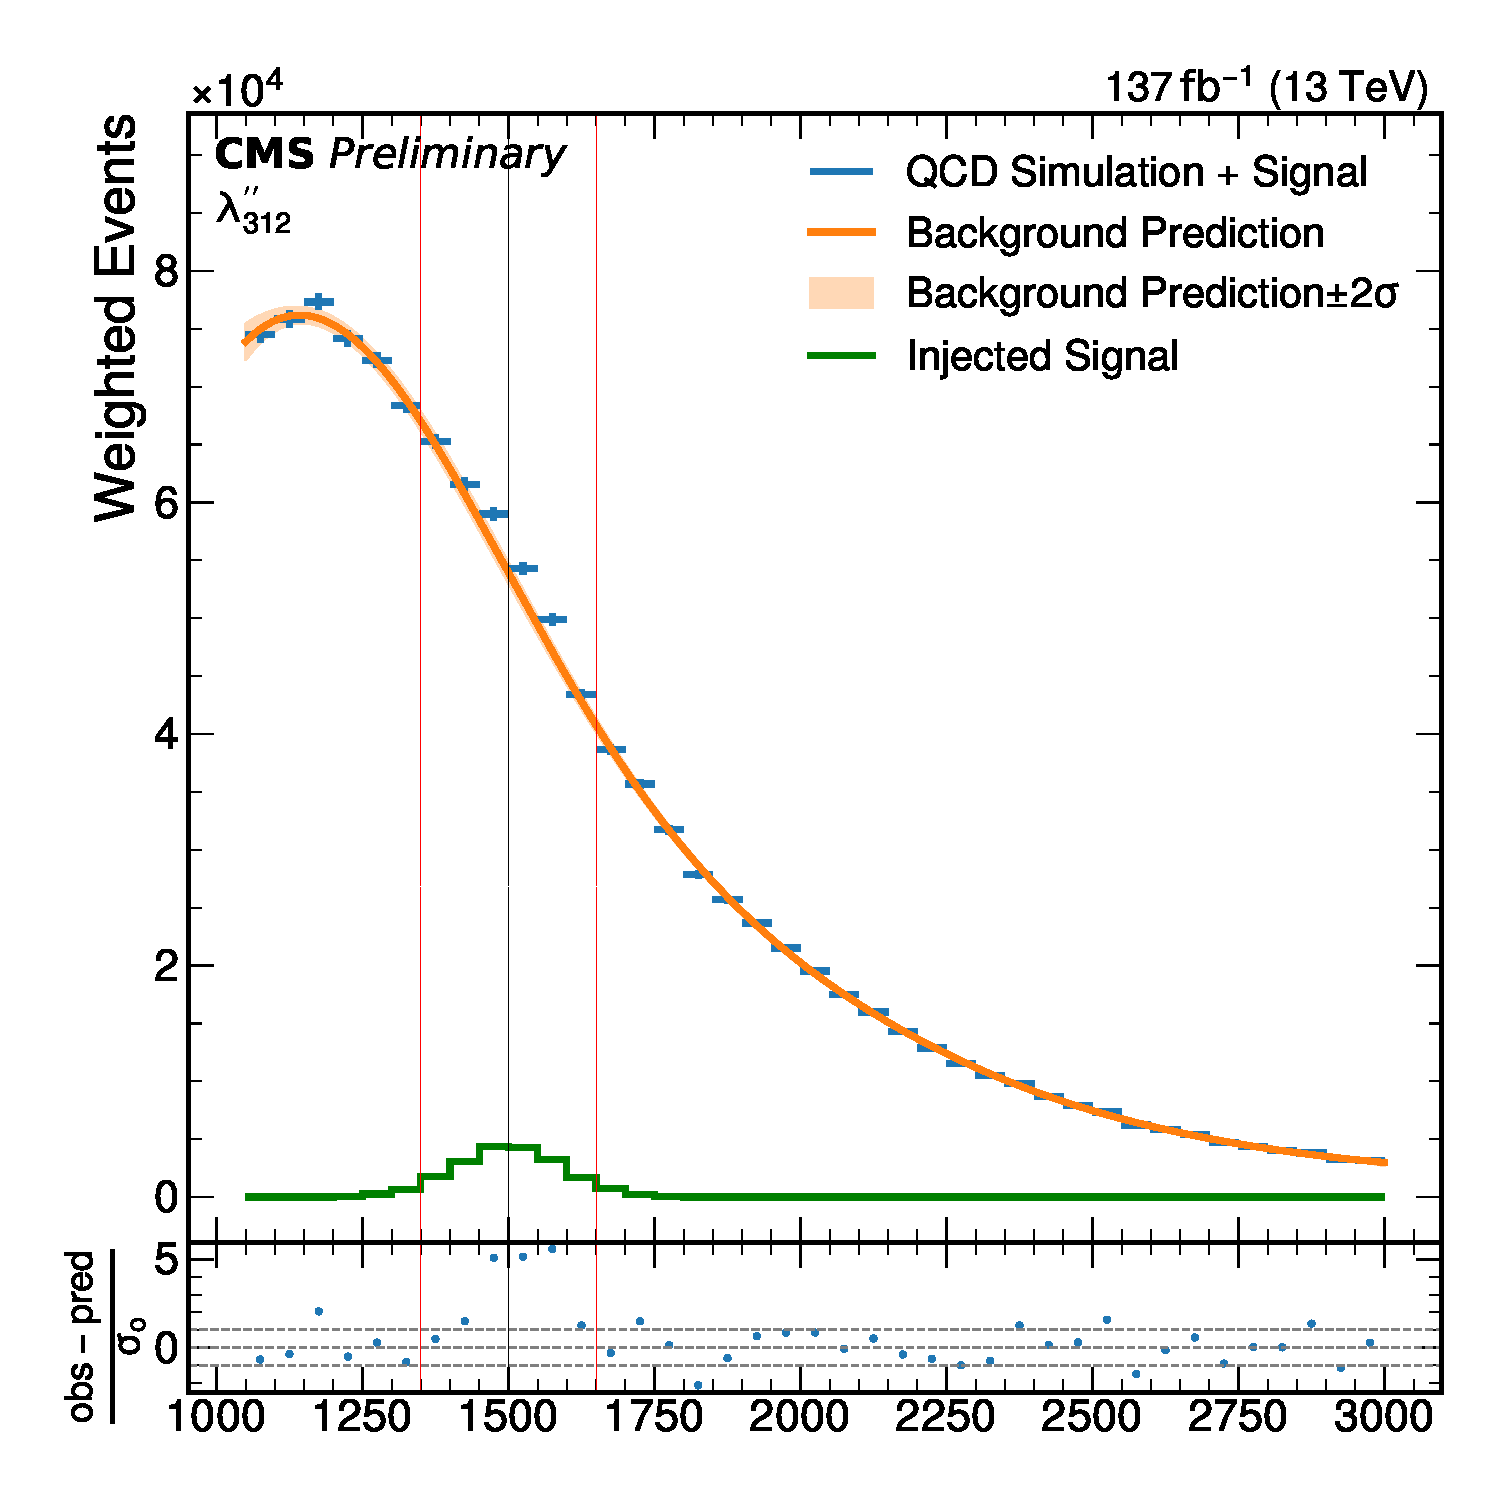
\includegraphics[width=0.31\textwidth]{figures/fitplots/pull_sr_inj_signal_312_1500_1400__lb1050__r15p0__fs_600p0__m1500p0_s90p0__w_1350p0_1650p0}}{}{}}{Scale = 600GeV}
%     \blockcite{\markimage{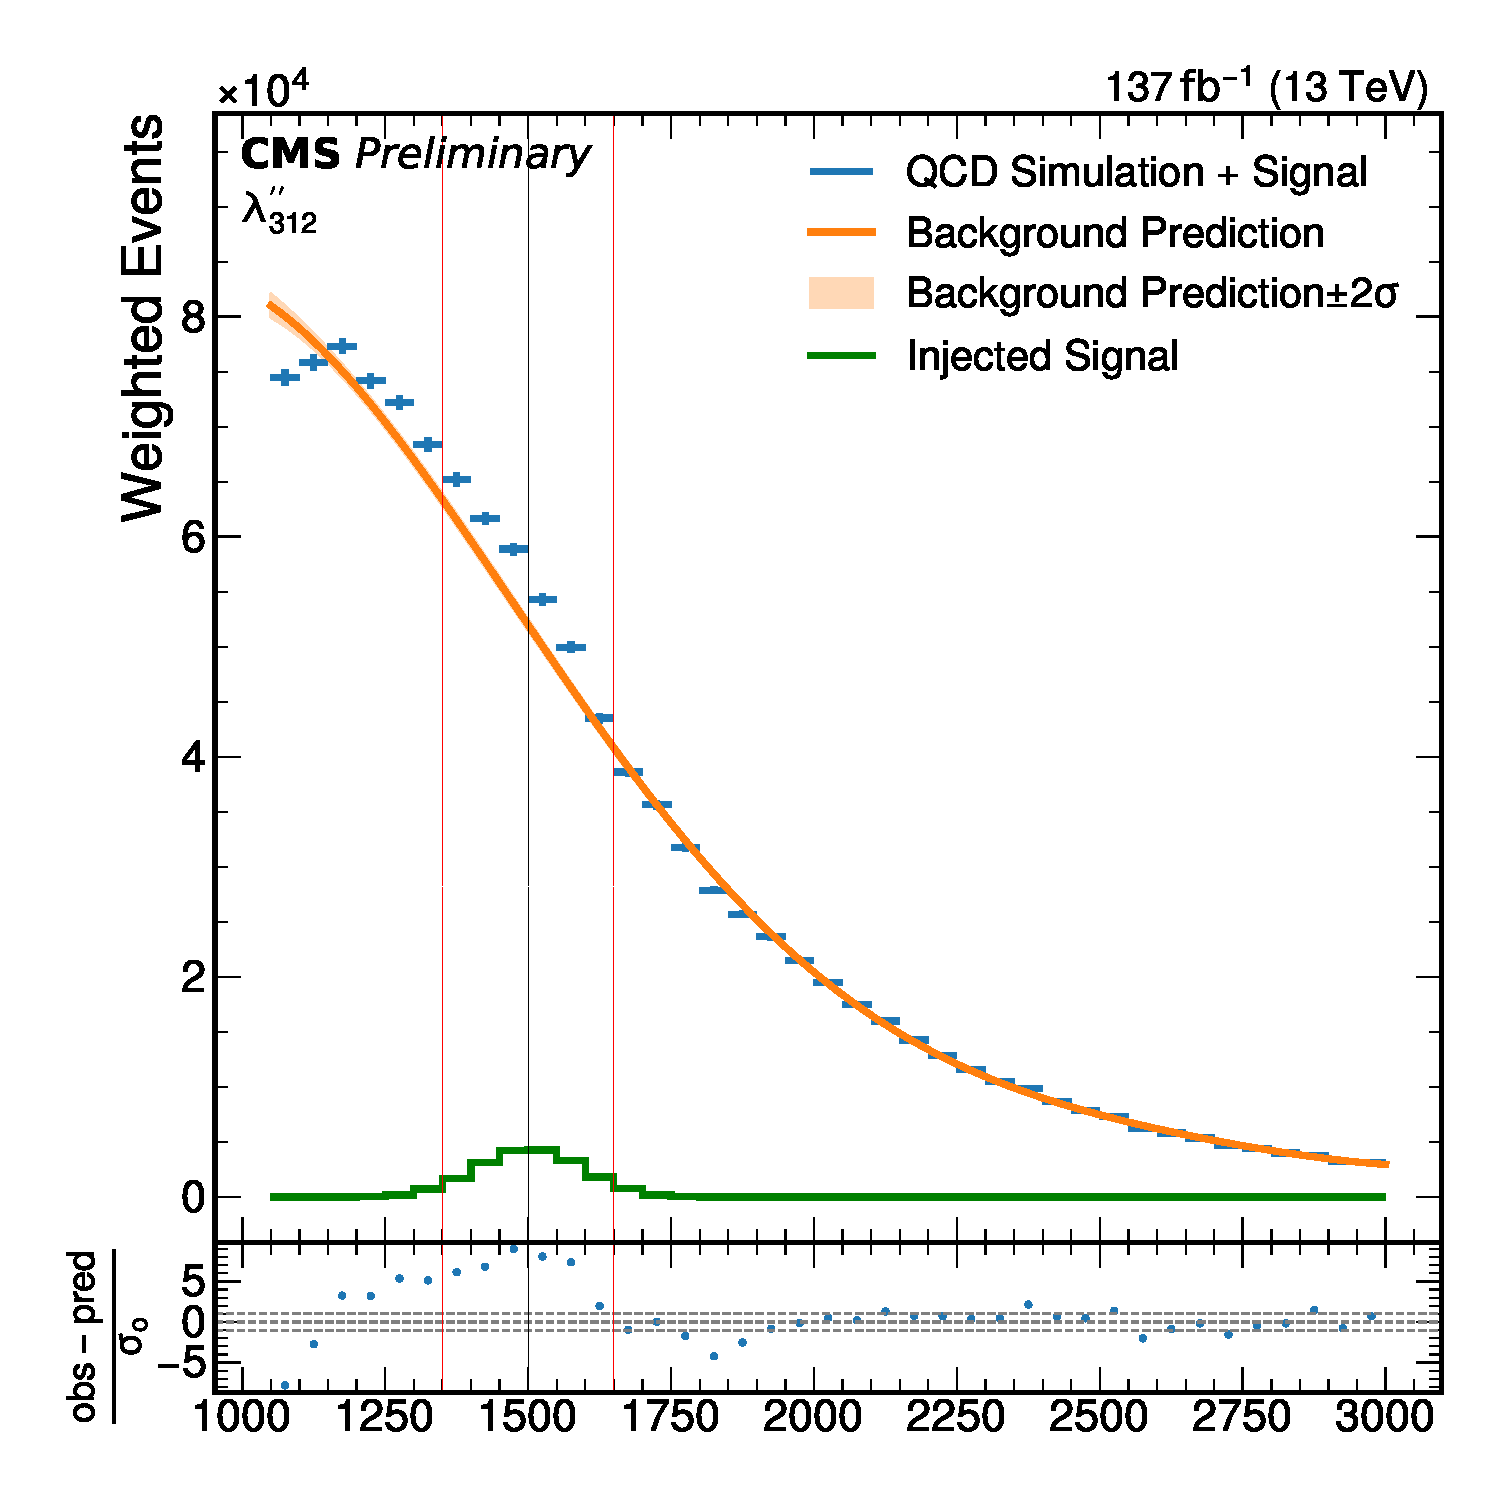
\includegraphics[width=0.31\textwidth]{figures/fitplots/pull_sr_inj_signal_312_1500_1400__lb1050__r15p0__fs_1350p0__m1500p0_s90p0__w_1350p0_1650p0}}{0.3,0.7}{ls2}}{Scale = 1350GeV}
%   \end{center}
%   \begin{onlyenv}<2>
%     \posannot[30:3cm]{ls1}{fill=UMNMaroon!10, draw=UMNMaroon}{Small length scales have have large \\uncertainties in their regressions.}
%     \posannot[210:3cm]{ls2}{fill=UMNMaroon!10, draw=UMNMaroon}{Long length scales can't accomodate local variations.}
%   \end{onlyenv}
% \end{frame}

\section[Regression Results]{2D Background Estimation With Gaussian Processes}
\label{sec:2d-gauss-proc}

\begin{frame}{Overview}
  \begin{itemize}
  \item We mask the region of space where the signal is expected, then use regression to estimate the background in the masked region.
  \item Hyperparameters are determined empirically.
  \item Both SR simulation and CR data have been examined. Background looks very similar in both cases. Here we present results with CR data to improve sample size. 
  \item Majority of studies have been focused on kernel selection and approximation techniques.
  \item All plots are over the plain background, with no signal injected.
  \end{itemize}
  \begin{center}
    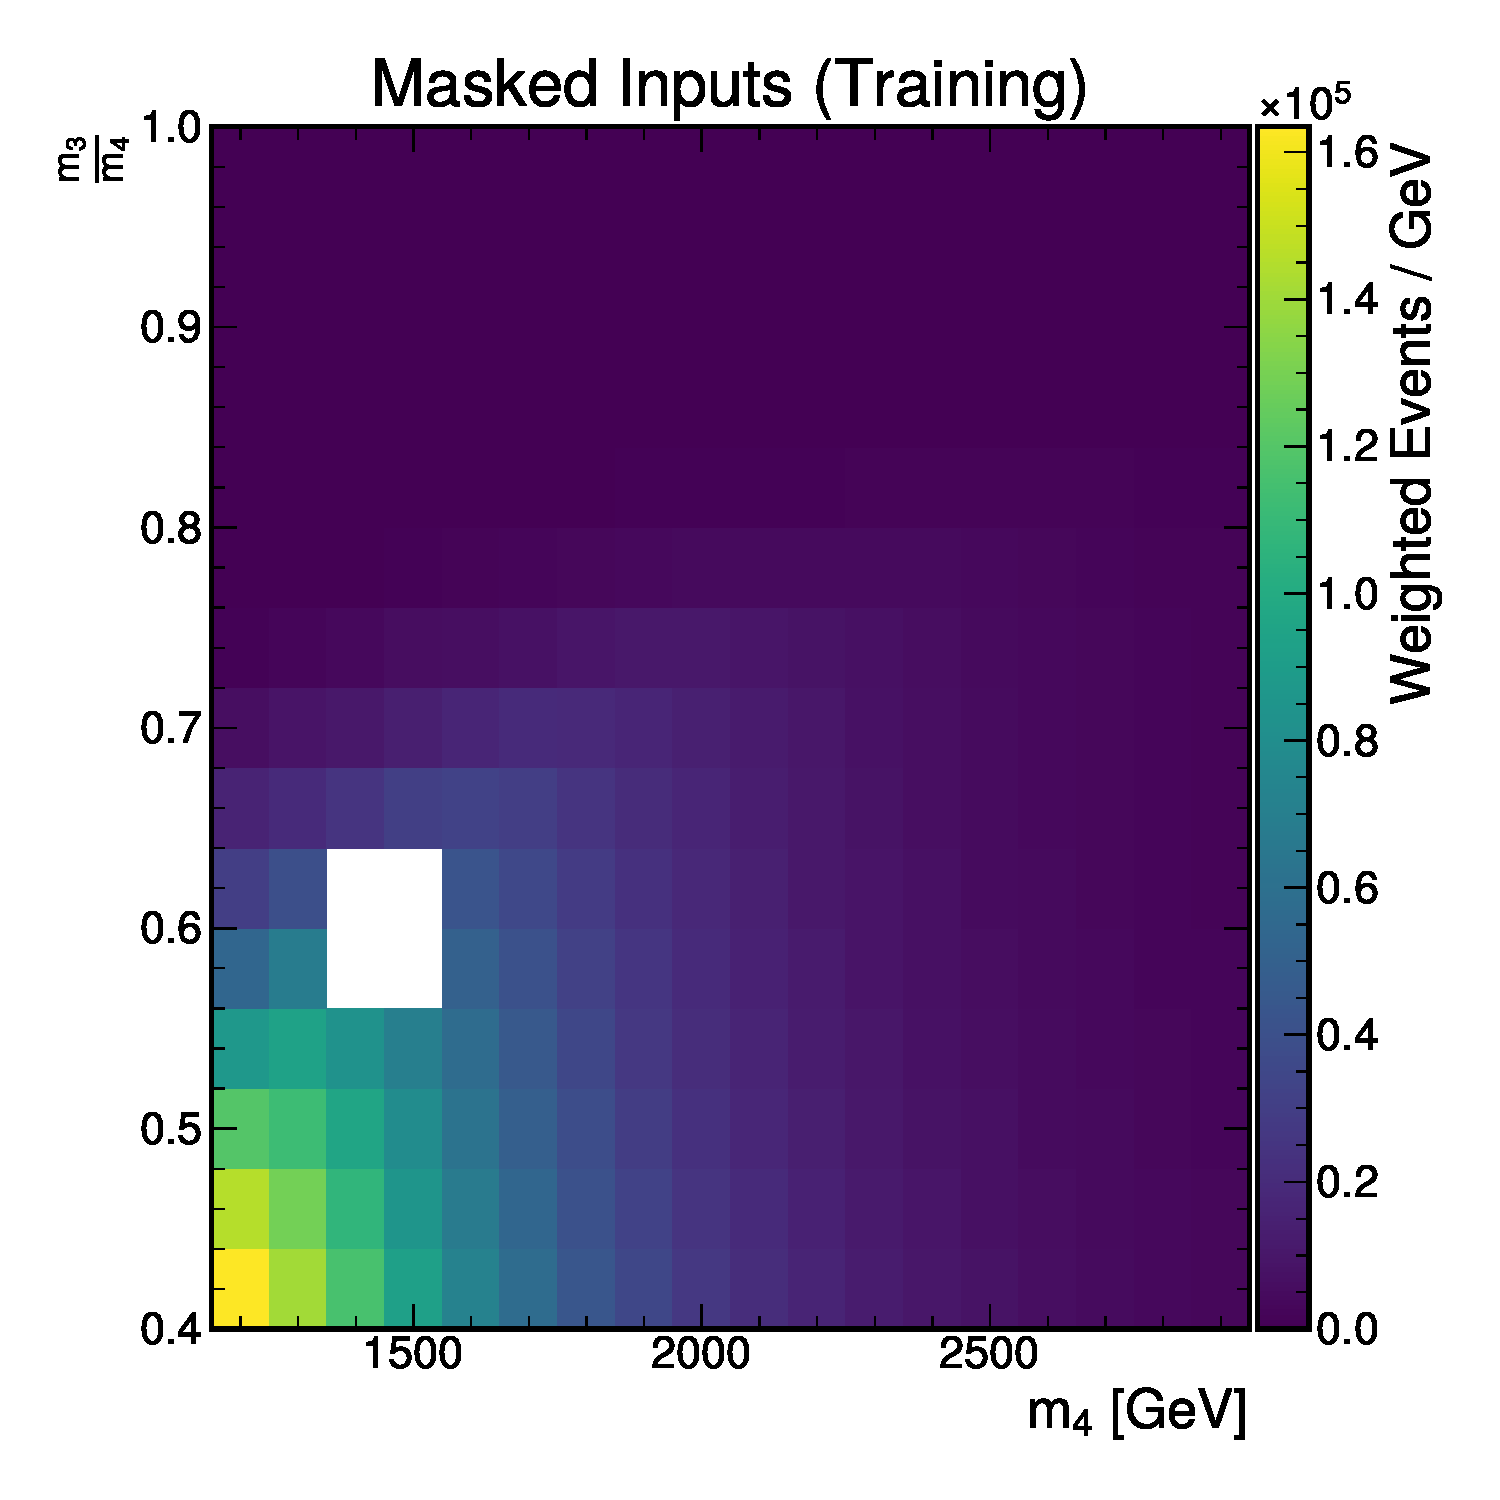
\includegraphics[width=0.3\textwidth]{figures/training_points}
  \end{center}
\end{frame}

\begin{frame}{Kernels in 2D}
  Multidimentional kernels can have a richer structure than 1D kernels. Below are several of the candidates used in our studies.
  \begin{itemize}
  \item Diagonal RBF (RBF)
    \begin{equation}
      k(\bm{x},\bm{x'}) = e^{ -\frac{1}{2} \left(  \bm{x} - \bm{x'}\right) D \left(  \bm{x} - \bm{x'}\right)}
    \end{equation}
    where $D$ is a diagonal matrix,
  \item General RBF (GRBF) kernel
    \begin{equation}
      k(\bm{x},\bm{x'}) = e^{ -\frac{1}{2} \left(  \bm{x} - \bm{x'}\right) M \left(  \bm{x} - \bm{x'}\right)}
    \end{equation}
    where $M$ is any positive semi-definite matrix.
  \item Feature Extractor RBF (NNRBF)
    \begin{equation}
      k(\bm{x},\bm{x'}) =  k_{RBF}(NN(\bm{x}),NN(\bm{x'}))
    \end{equation}
    where $NN$ is an simple neural network ``feature extractor''.
  \end{itemize}
\end{frame}


\begin{frame}{Full Plane Fit With RBF}
  \begin{center}
    \begin{onlyenv}<1>
      \begin{annotimage}{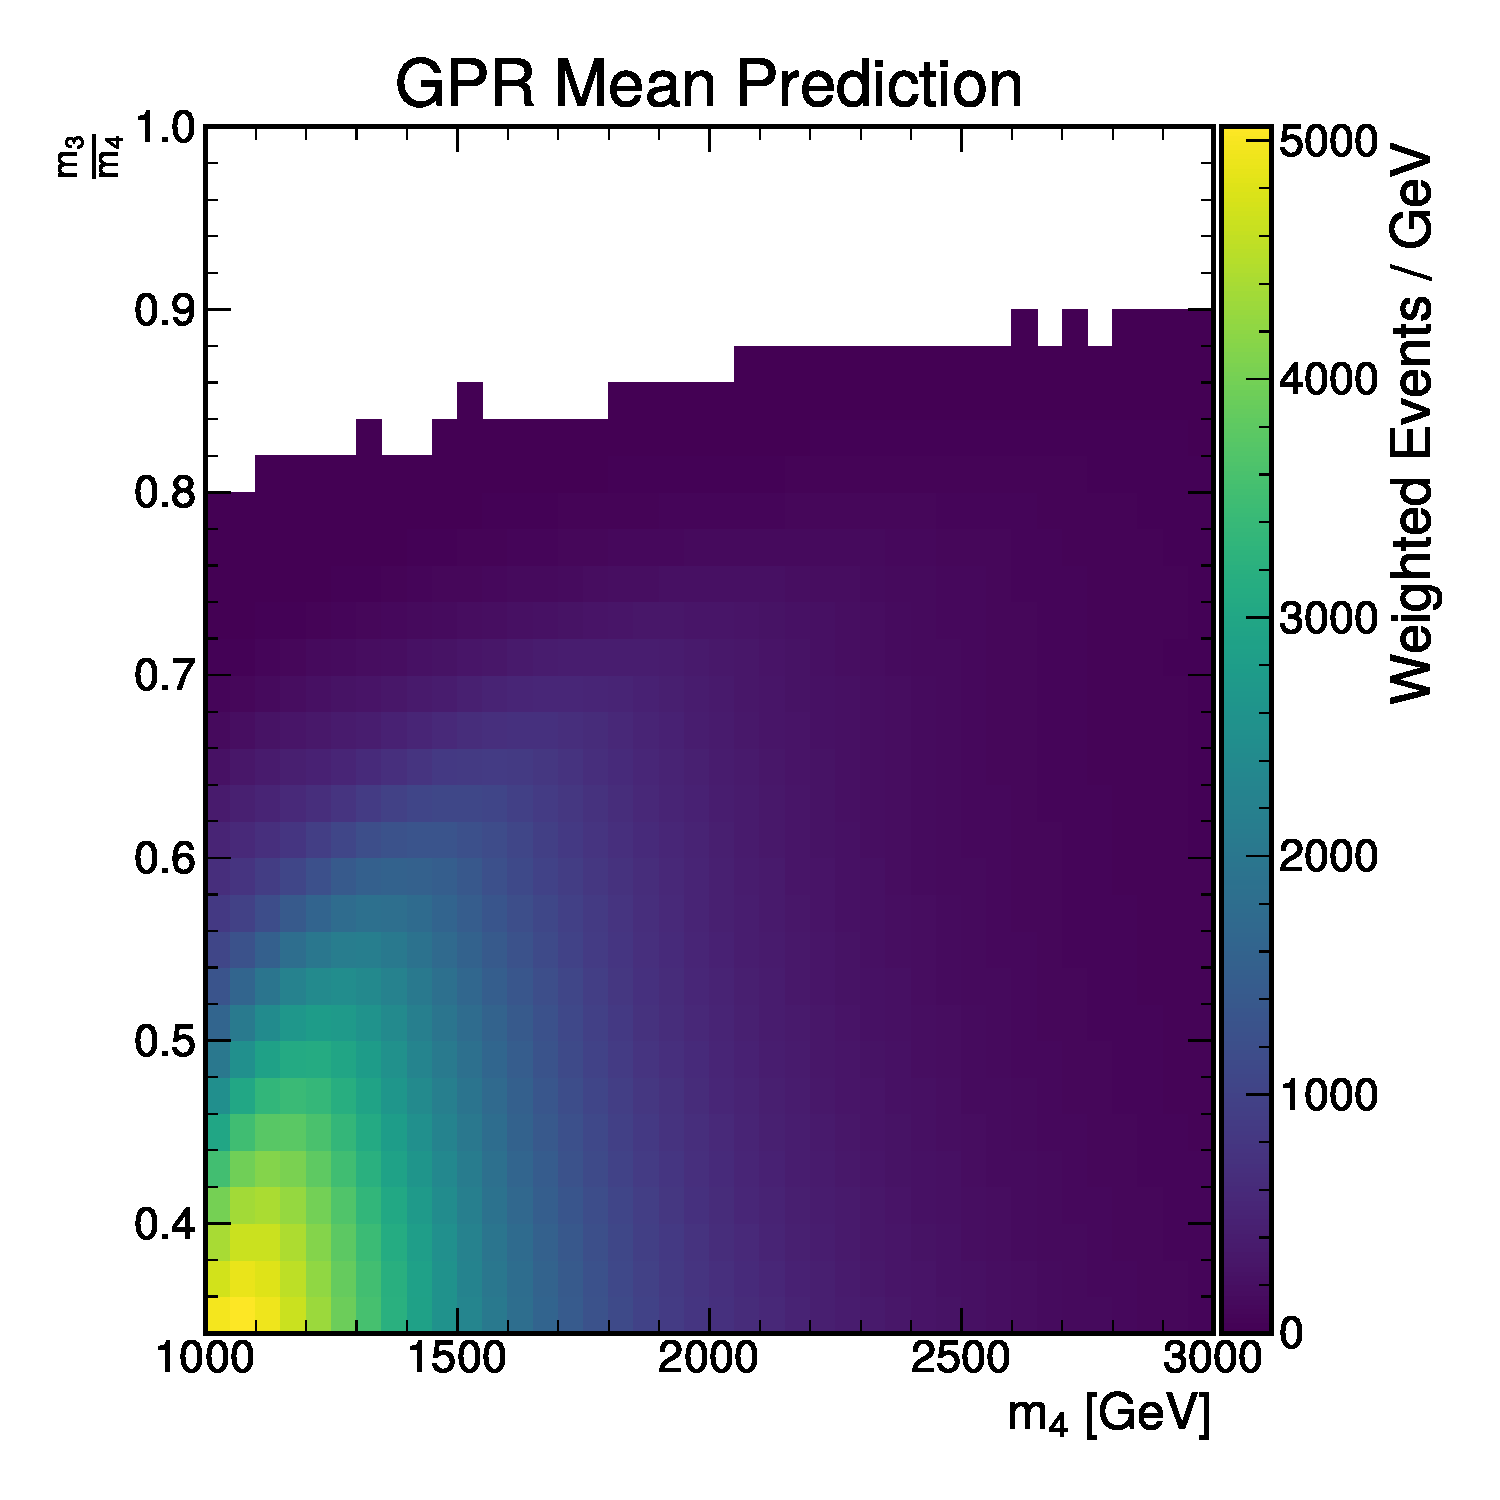
\includegraphics[width=0.45\textwidth]{figures/rbf_gp_mean.pdf}}
      \end{annotimage}
      \begin{annotimage}{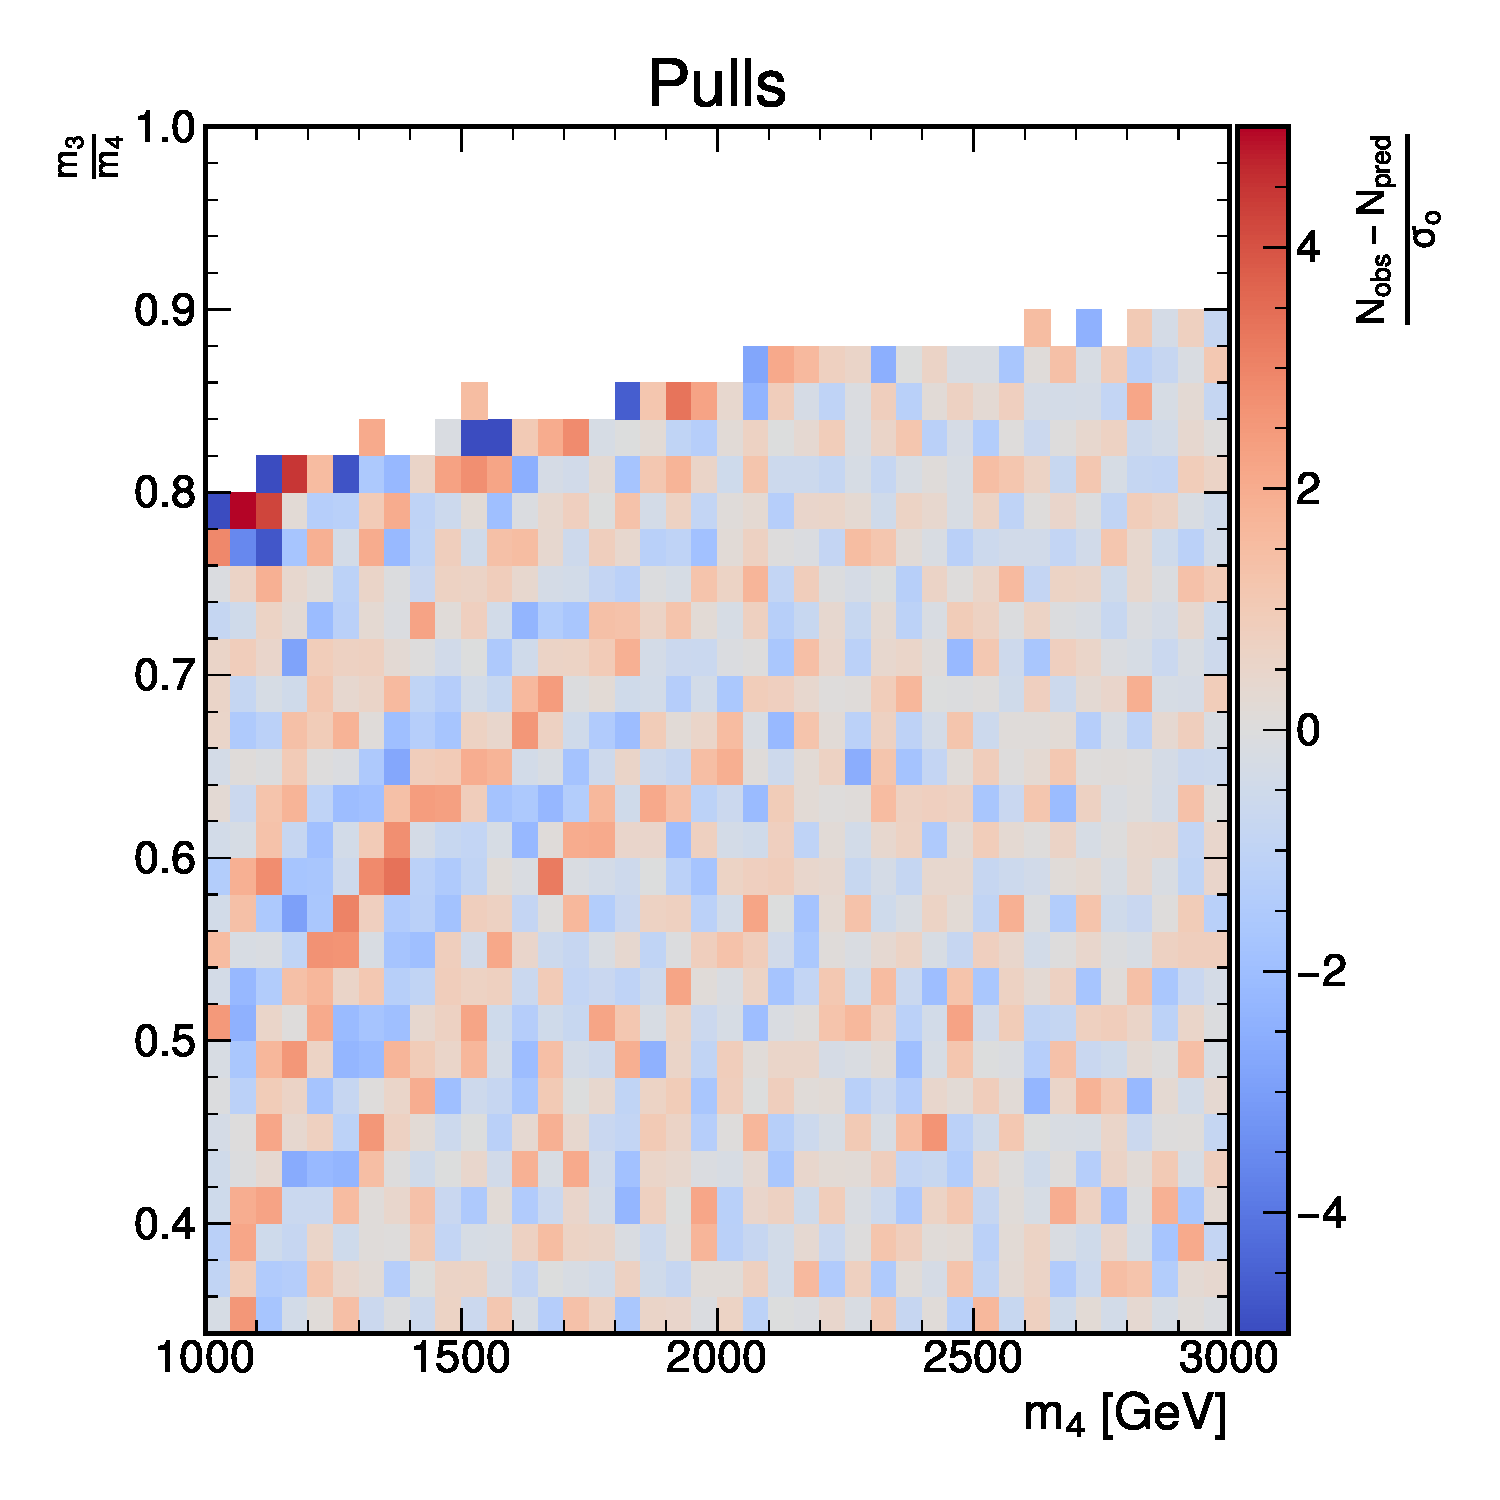
\includegraphics[width=0.45\textwidth]{figures/2dpullplots/rbf/NoWindow.pdf}}
      \end{annotimage}
    \end{onlyenv}
    % \begin{onlyenv}<2>
    %   \begin{annotimage}{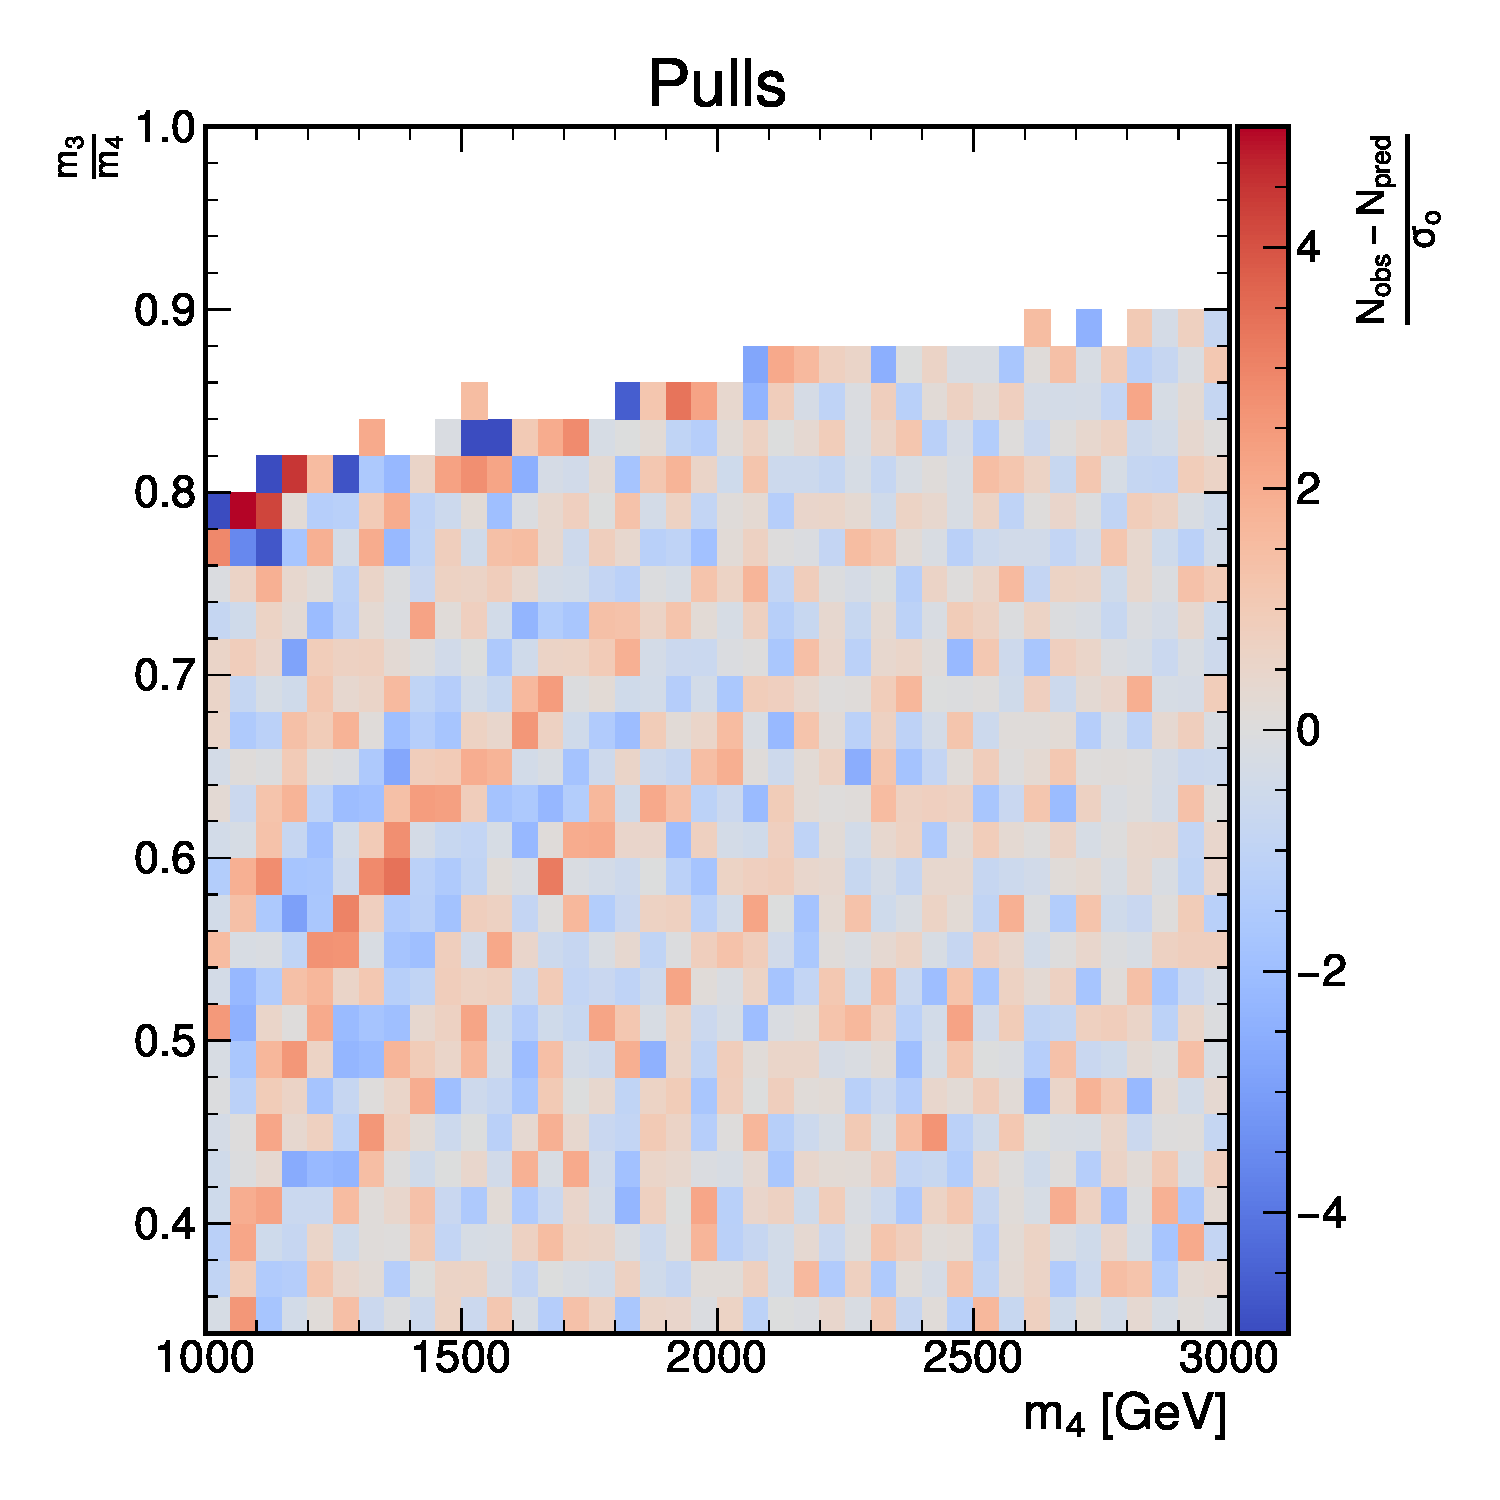
\includegraphics[width=0.65\textwidth]{figures/2dpullplots/rbf/NoWindow.pdf}}
    %   \end{annotimage}
    % \end{onlyenv}
  \end{center}
\end{frame}


\newcommand{\makegrid}[6]{
  \begin{center}
    \blockcite[(0,1em)]{#1}{$m_{\stopq}=1200\,,\,m_{\chi}=600$}
    \blockcite[(0,1em)]{#2}{$m_{\stopq}=1500\,,\,m_{\chi}=750$}
    \blockcite[(0,1em)]{#3}{$m_{\stopq}=1500\,,\,m_{\chi}=750$}
  \end{center}
  \begin{center}
    \blockcite[(0,1em)]{#4}{$m_{\stopq}=1500\,,\,m_{\chi}=750$}
    \blockcite[(0,1em)]{#5}{$m_{\stopq}=2000\,,\,m_{\chi}=1400$}
    \blockcite[(0,1em)]{#6}{$m_{\stopq}=2000\,,\,m_{\chi}=1000$}
  \end{center}

}

\begin{frame}{Fit Using Diagonal RBF}
  \makegrid%
  {\markimage{\includegraphics[width=0.3\textwidth]{figures/2dpullplots/rbf/E_1200_0p5_100_0p05.pdf}}{0.3,0.5}{rbf2}}%
  {\includegraphics[width=0.3\textwidth]{figures/2dpullplots/rbf/E_1500_0p5_100_0p05.pdf}}%
  {\includegraphics[width=0.3\textwidth]{figures/2dpullplots/rbf/E_1500_0p5_150_0p05.pdf}}%
  {\markimage{\includegraphics[width=0.3\textwidth]{figures/2dpullplots/rbf/E_1500_0p5_150_0p07.pdf}}{0.3,0.3}{rbf1} }%
  {\includegraphics[width=0.3\textwidth]{figures/2dpullplots/rbf/E_2000_0p7_150_0p05.pdf}}%
  {\includegraphics[width=0.3\textwidth]{figures/2dpullplots/rbf/E_2000_0p5_150_0p07.pdf}}%
  \begin{onlyenv}<2>
    \posannot[20:3]{rbf1}{fill=UMNMaroon!10, draw=UMNMaroon}{Poor pulls near complex regions \\ because correlation structure is ignored.}
    \posannot[-20:3]{rbf2}{fill=UMNMaroon!10, draw=UMNMaroon}{Ridge region results in ``waves'' of poor pulls.}
  \end{onlyenv}
\end{frame}

\begin{frame}{Fit Using GRBF}
  \makegrid%
  {\markimage{\includegraphics[width=0.3\textwidth]{figures/2dpullplots/grbf/E_1200_0p5_100_0p05.pdf}}{0.3,0.5}{grbf1}}%
  {\includegraphics[width=0.3\textwidth]{figures/2dpullplots/grbf/E_1500_0p5_100_0p05.pdf}}%
  {\includegraphics[width=0.3\textwidth]{figures/2dpullplots/grbf/E_1500_0p5_150_0p05.pdf}}%
  {\markimage{\includegraphics[width=0.3\textwidth]{figures/2dpullplots/grbf/E_1500_0p5_150_0p07.pdf}}{0.3,0.3}{grbf2} }%
  {\includegraphics[width=0.3\textwidth]{figures/2dpullplots/grbf/E_2000_0p7_150_0p05.pdf}}%
  {\includegraphics[width=0.3\textwidth]{figures/2dpullplots/grbf/E_2000_0p5_150_0p07.pdf}}%
  \begin{onlyenv}<2>
    \posannot[20:3]{grbf2}{fill=UMNMaroon!10, draw=UMNMaroon}{Allowing off-diagonal terms improved pulls.}
    \posannot[-20:3]{grbf1}{fill=UMNMaroon!10, draw=UMNMaroon}{Ridge behavior is reduced.}
  \end{onlyenv}
\end{frame}

% \begin{frame}{Fit Using Small Deep Kernel}
%   \begin{center}
%     \includegraphics[width=0.3\textwidth]{figures/2dpullplots/nnrbf_16_8/E_1200_0p5_100_0p05.pdf} 
%     \includegraphics[width=0.3\textwidth]{figures/2dpullplots/nnrbf_16_8/E_1500_0p5_100_0p05.pdf} 
%     \includegraphics[width=0.3\textwidth]{figures/2dpullplots/nnrbf_16_8/E_1500_0p5_150_0p05.pdf} 
%     \includegraphics[width=0.3\textwidth]{figures/2dpullplots/nnrbf_16_8/E_1500_0p5_150_0p07.pdf} 
%     \includegraphics[width=0.3\textwidth]{figures/2dpullplots/nnrbf_16_8/E_2000_0p7_150_0p05.pdf} 
%     \includegraphics[width=0.3\textwidth]{figures/2dpullplots/nnrbf_16_8/E_2000_0p5_150_0p07.pdf} 
%   \end{center}
% \end{frame}

\begin{frame}{Fit Using ANN Augmented RBF}
  \makegrid%
  {\markimage{\includegraphics[width=0.3\textwidth]{figures/2dpullplots/nnrbf_32_16_8/E_1200_0p5_100_0p05.pdf}}{0.3,0.5}{nnrbf_32_16_81}}%
  {\includegraphics[width=0.3\textwidth]{figures/2dpullplots/nnrbf_32_16_8/E_1500_0p5_100_0p05.pdf}}%
  {\includegraphics[width=0.3\textwidth]{figures/2dpullplots/nnrbf_32_16_8/E_1500_0p5_150_0p05.pdf}}%
  {\markimage{\includegraphics[width=0.3\textwidth]{figures/2dpullplots/nnrbf_32_16_8/E_1500_0p5_150_0p07.pdf}}{0.3,0.3}{nnrbf_32_16_82} }%
  {\includegraphics[width=0.3\textwidth]{figures/2dpullplots/nnrbf_32_16_8/E_2000_0p7_150_0p05.pdf}}%
  {\includegraphics[width=0.3\textwidth]{figures/2dpullplots/nnrbf_32_16_8/E_2000_0p5_150_0p07.pdf}}%

  \begin{onlyenv}<2>
    \begin{beamerpopover}
      \begin{block}{}
        Kernel with an ANN feature extractor can eliminate the ridge behavior while still providing good predictive performance. 
      \end{block}
    \end{beamerpopover}
  \end{onlyenv}
\end{frame}


\begin{frame}{Covariances}
  \begin{onlyenv}<1>
    \begin{splitcol}[0.65]
      \begin{col}
        \begin{itemize}
        \item We can examine the actual posterior covariance of the gaussian process to get a better sense of what the kernel is learning.
        \item See how the more advanced kernels better take in to account the background shape.
        \item Below shows how the center of the blinding window, shown in red, covaries with all other points in the plane.
        \end{itemize}
      \end{col}
      \begin{col}
        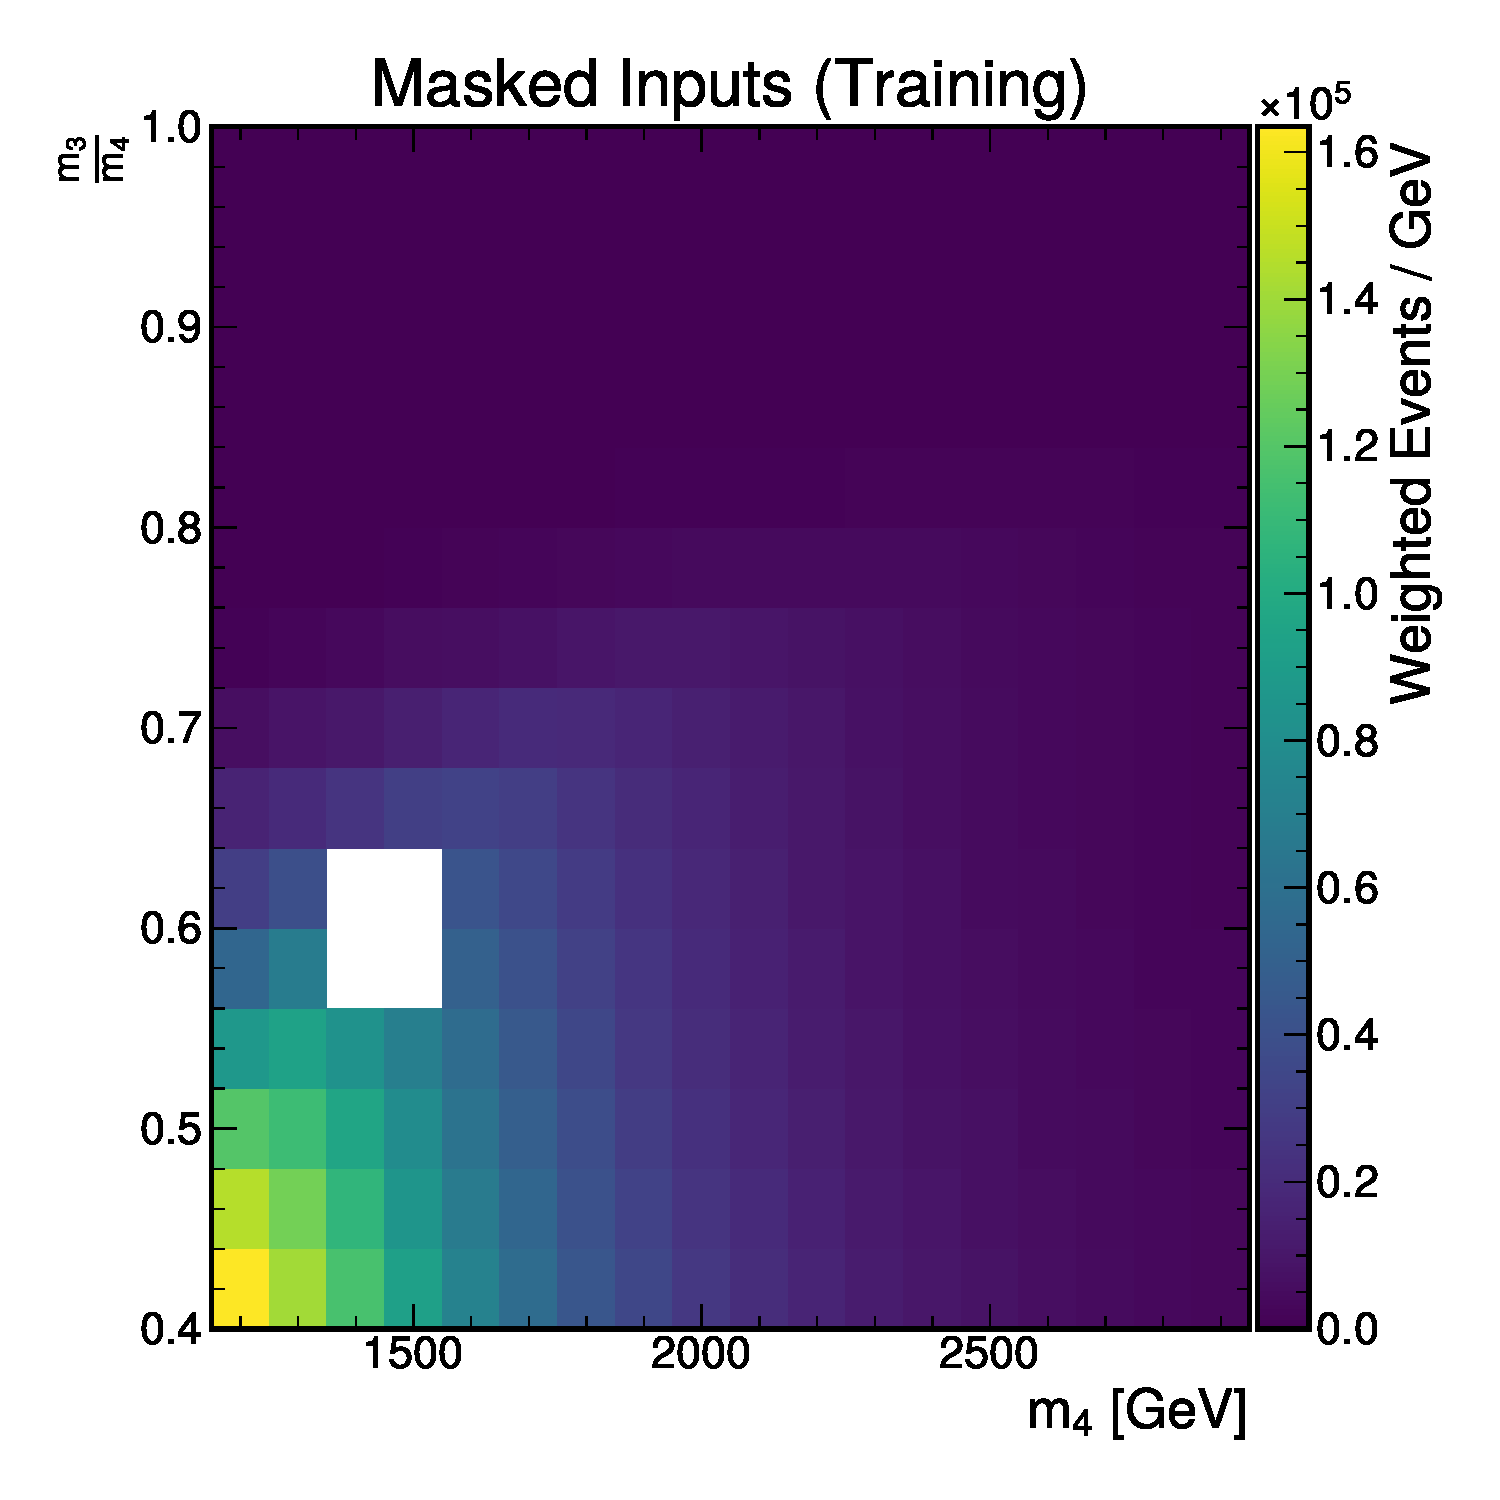
\includegraphics[width=1.0\textwidth]{figures/training_points}
      \end{col}
    \end{splitcol}
  \end{onlyenv}
  \begin{onlyenv}<2>
    \begin{center}
      \begin{annotimage}{\includegraphics[width=0.30\textwidth]{figures/2dpullplots/rbf/E_1500_0p5_150_0p07.pdf}}
        \node[anchor=west] at (0.14,0.83) {\tiny RBF};
      \end{annotimage}
      \begin{annotimage}{\includegraphics[width=0.30\textwidth]{figures/2dpullplots/grbf/E_1500_0p5_150_0p07.pdf}}
        \node[anchor=west] at (0.14,0.83) {\tiny GRBF};
      \end{annotimage}
      \begin{annotimage}{\includegraphics[width=0.30\textwidth]{figures/2dpullplots/nnrbf_32_16_8/E_1500_0p5_150_0p07.pdf}}
        \node[anchor=west] at (0.14,0.83) {\tiny NNRBF};
      \end{annotimage}
    \end{center}
  \end{onlyenv}
  \begin{onlyenv}<1-2>
    \begin{center}
      \vspace{-0.6cm}
      \begin{annotimage}{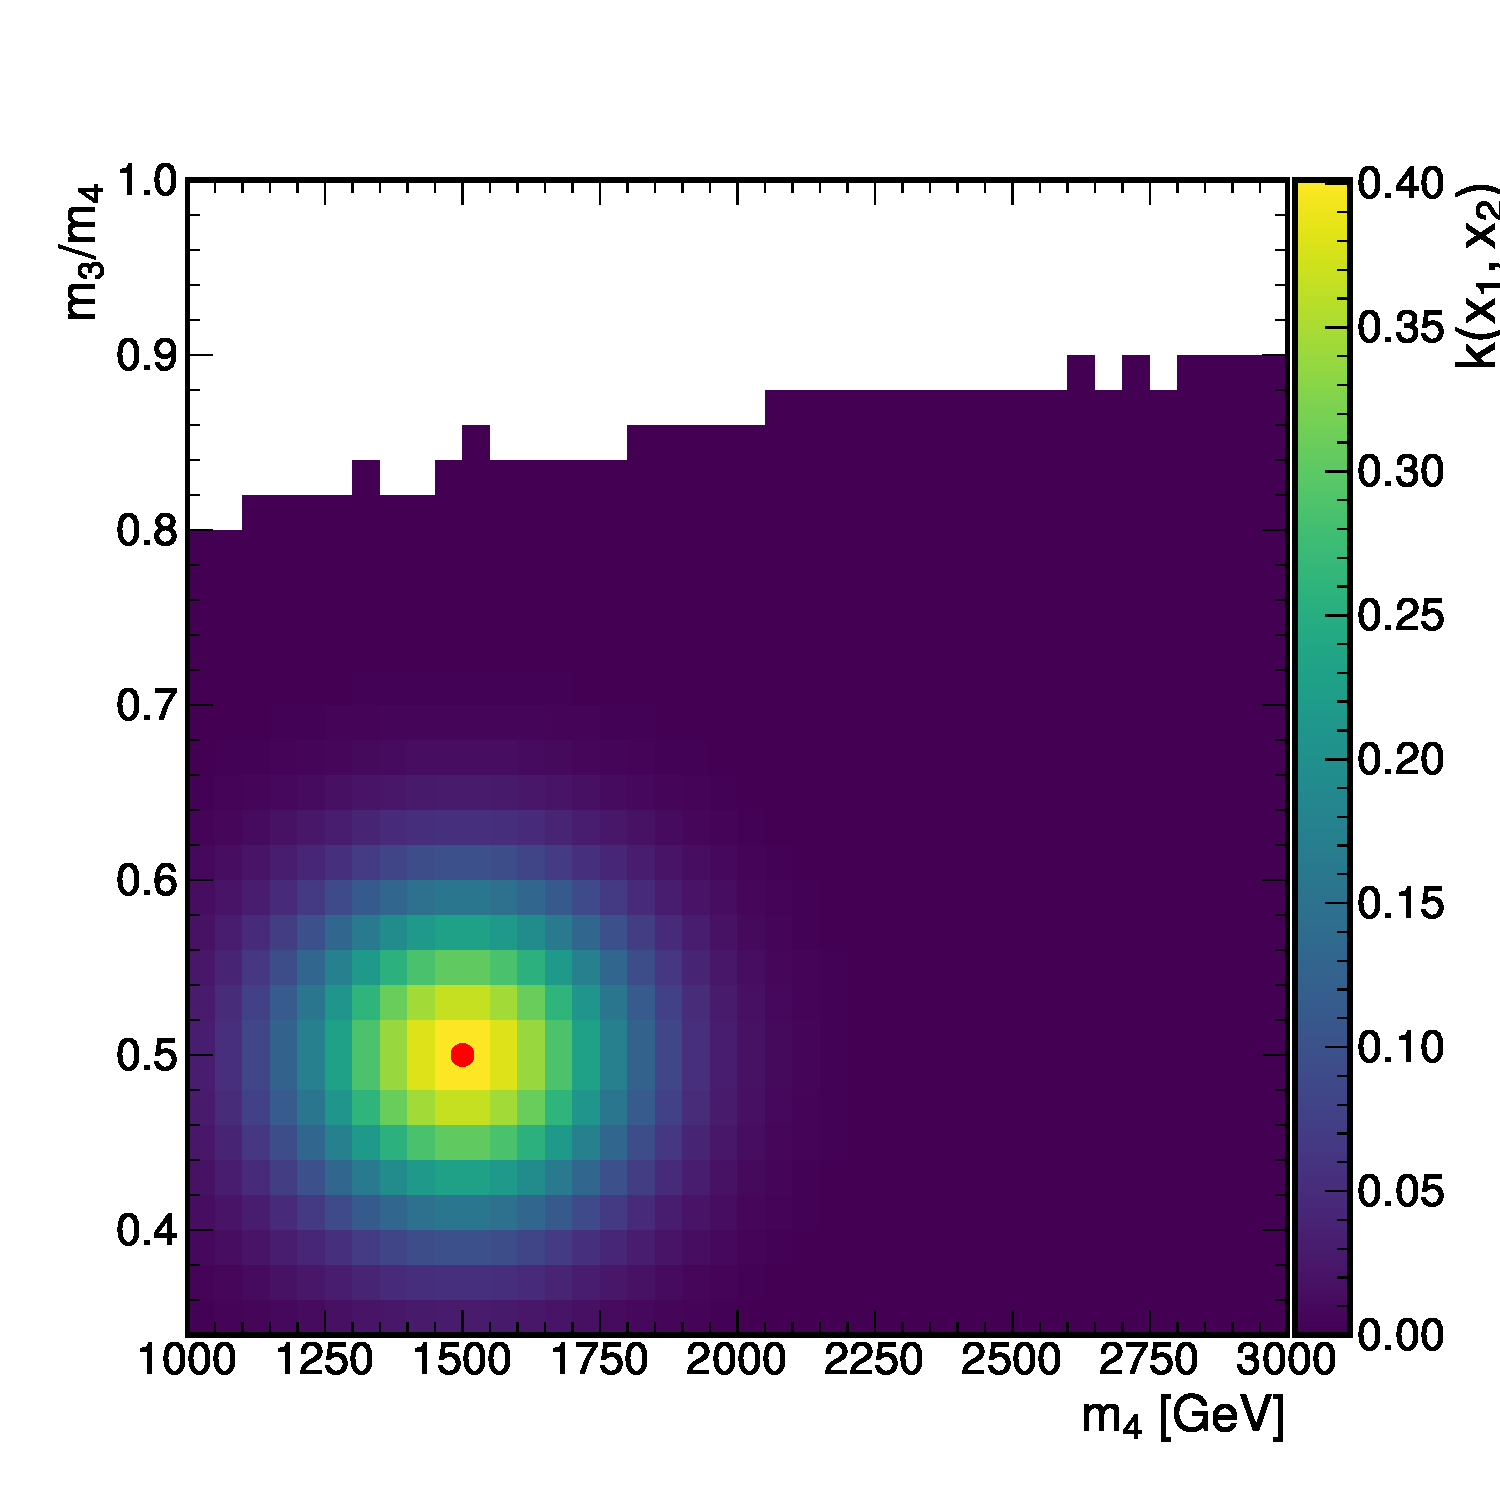
\includegraphics[width=0.30\textwidth]{figures/covars/rbf_E_1500_0p5_150_0p07.pdf}}
        \node[anchor=west] at (0.12,0.8) {\tiny RBF};
      \end{annotimage}
      \begin{annotimage}{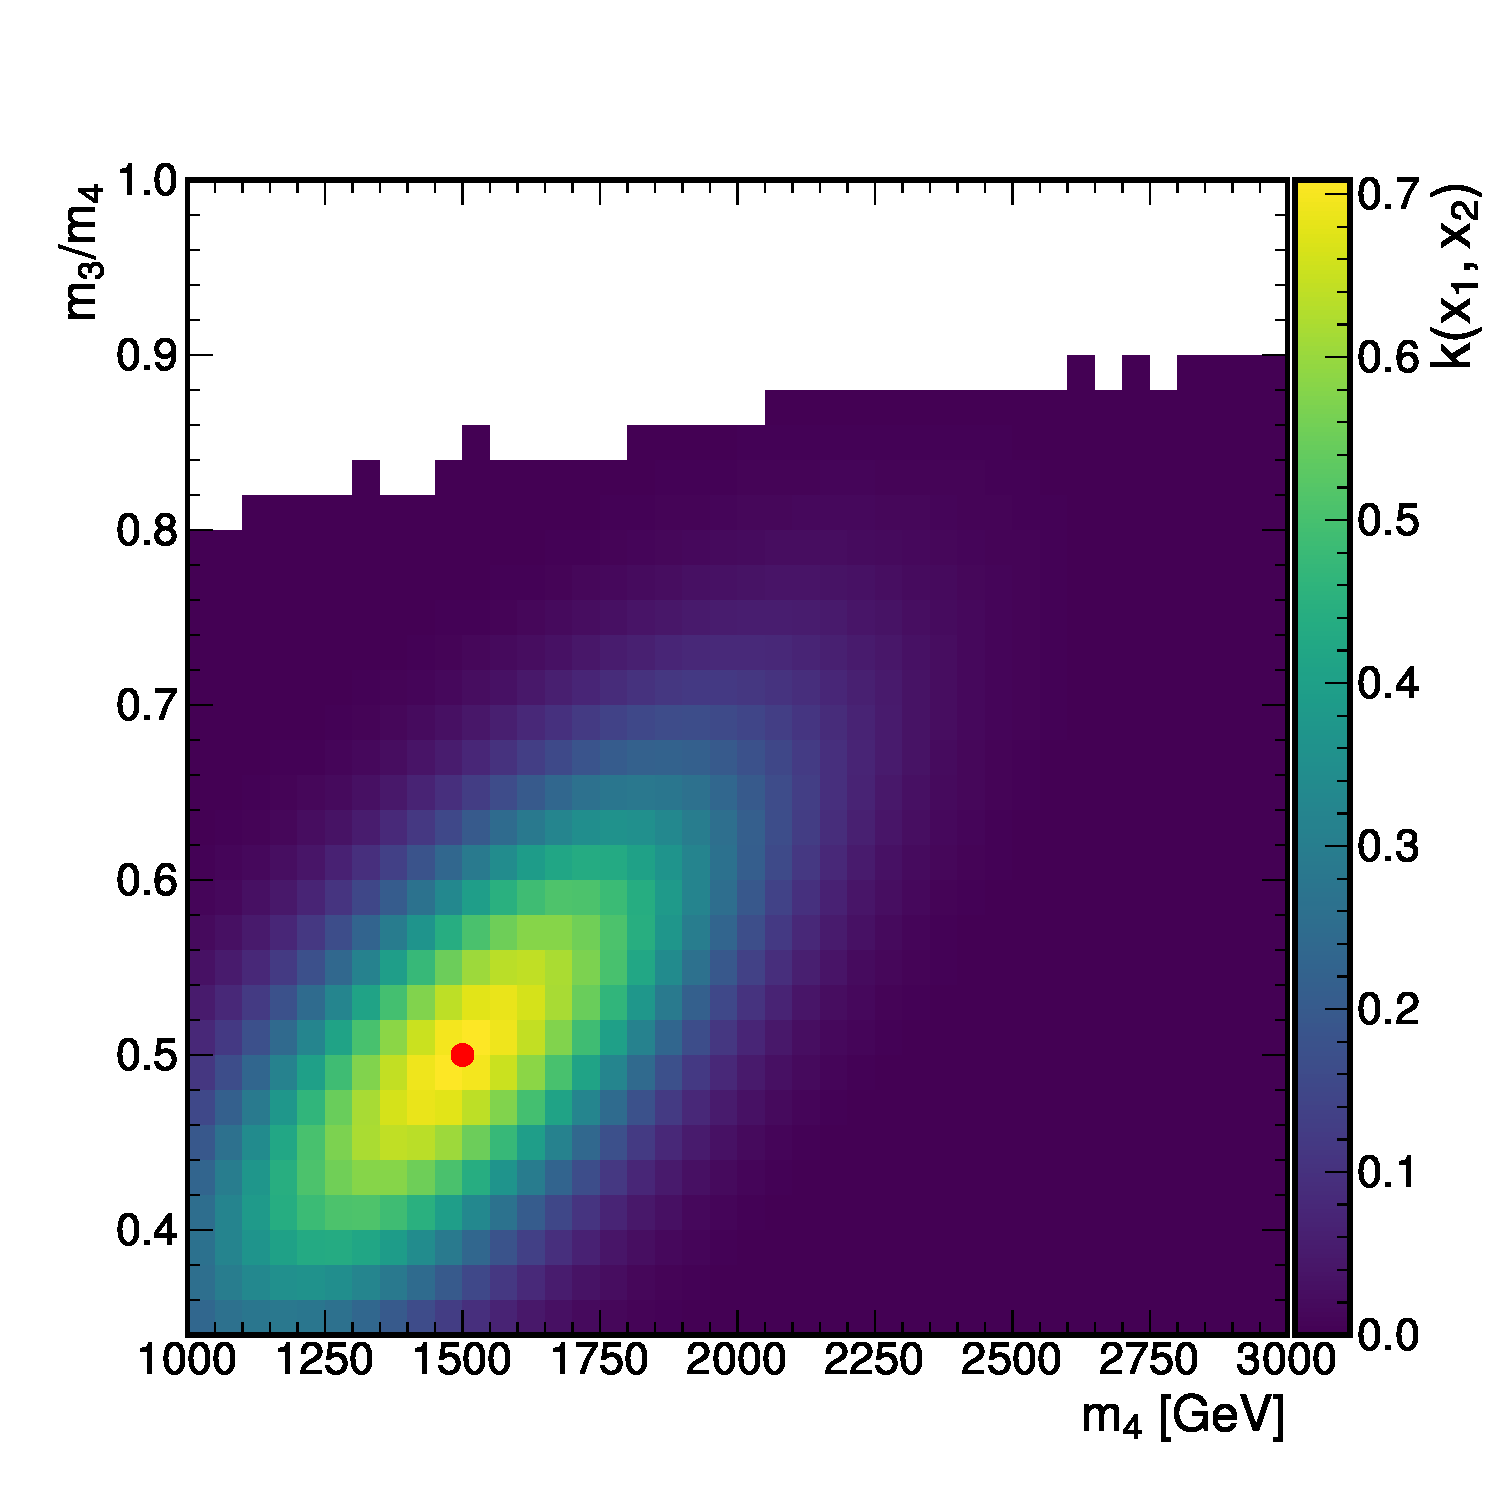
\includegraphics[width=0.30\textwidth]{figures/covars/grbf_E_1500_0p5_150_0p07.pdf}}
        \node[anchor=west] at (0.12,0.8) {\tiny GRBF};
      \end{annotimage}
      \begin{annotimage}{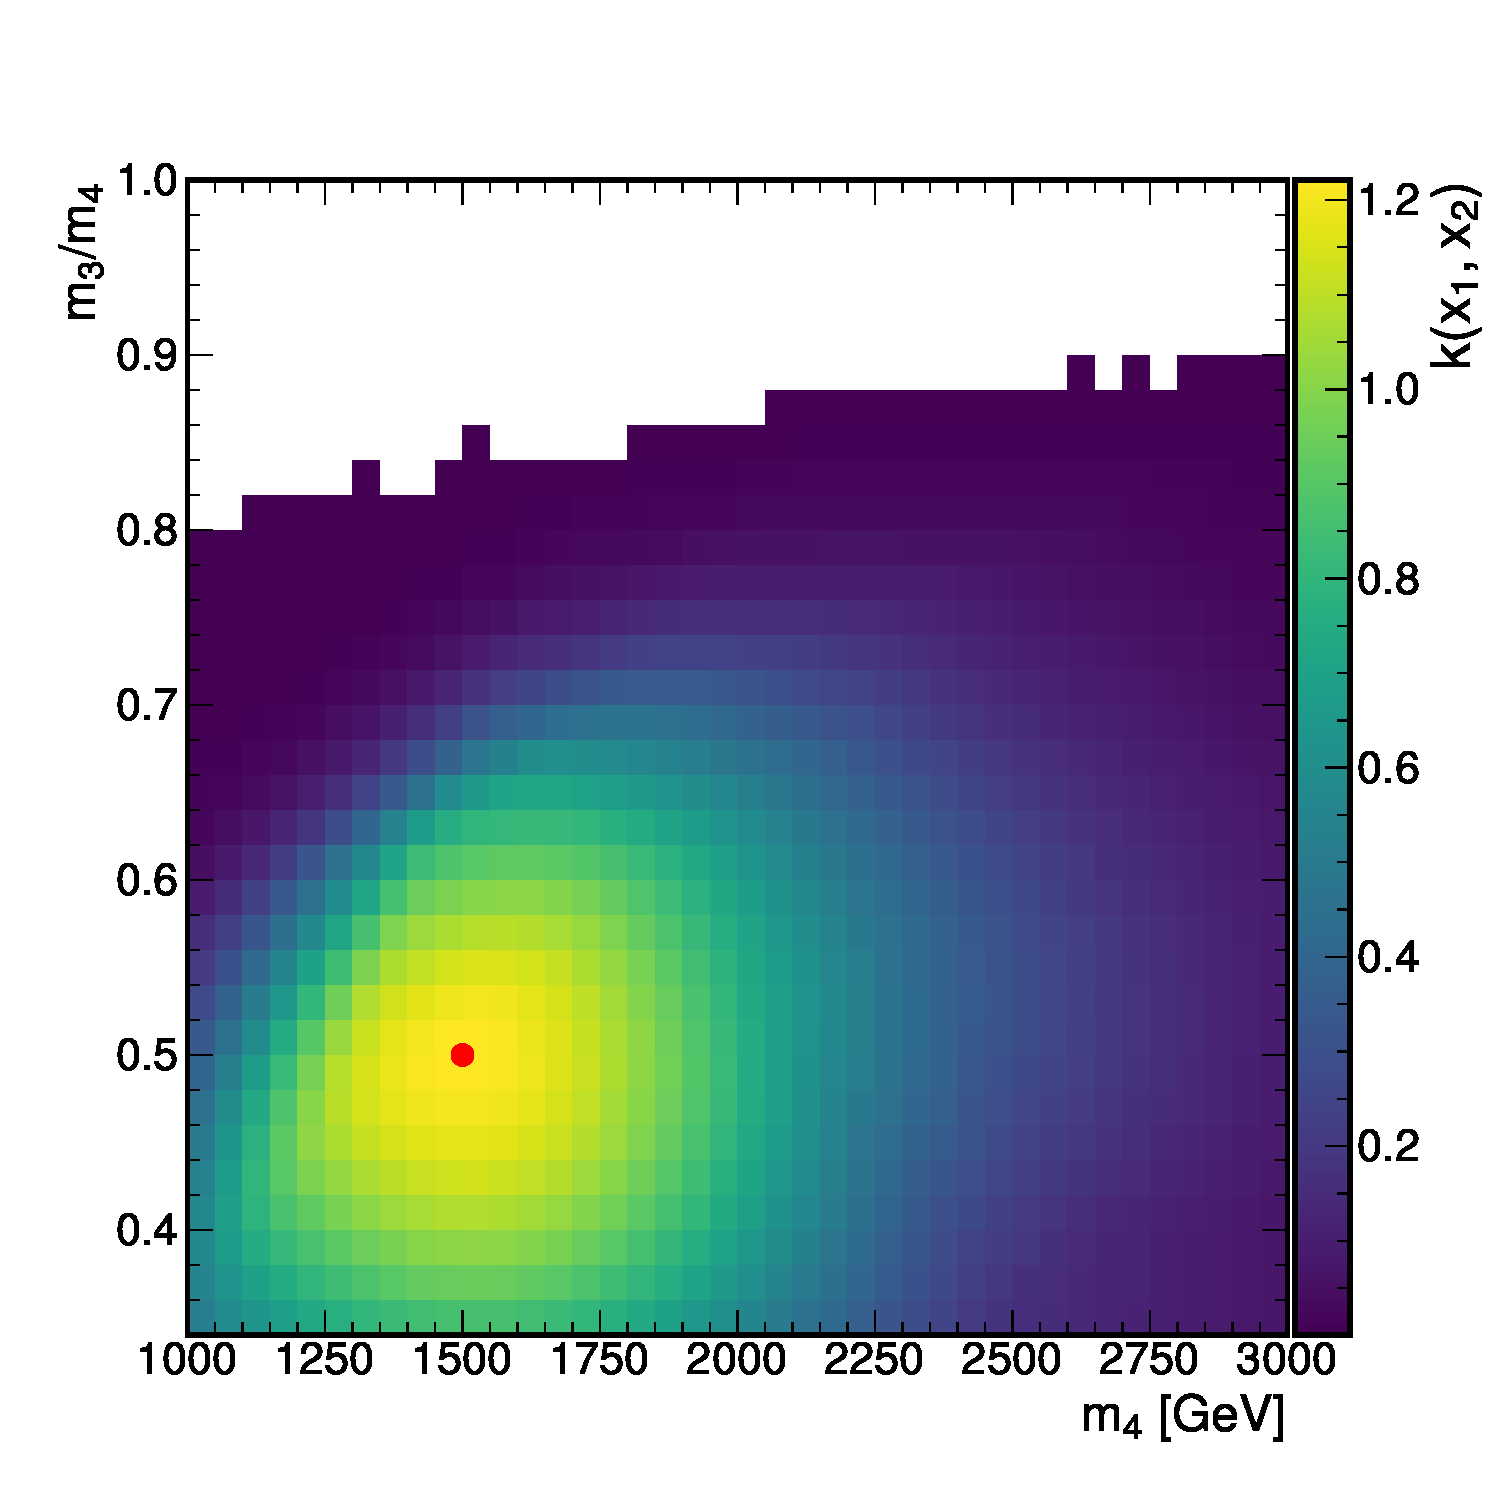
\includegraphics[width=0.30\textwidth]{figures/covars/nnrbf_32_16_8_E_1500_0p5_150_0p07.pdf}}
        \node[anchor=west] at (0.12,0.8) {\tiny NNRBF};
      \end{annotimage}
    \end{center}
  \end{onlyenv}

  
\end{frame}


\section[Statistical Considerations]{Preliminary Statistical Strategy and Inquiries}


\begin{frame}{Strategy Overview}
  \begin{onlyenv}<1>
    \begin{block}{}
      We see that GPR can provide a good estimate of the background over a wide range of blinding windows. How can we use this to extract signal and set limits?
    \end{block}
  \end{onlyenv}
  \begin{onlyenv}<1-2>
    \begin{enumerate}
    \item Determine appropriate kernel form using MC and CR Data. We will derive a systematic to account for differences between regions for the kernel choice.
    \item For each signal, use MC to determine blinding window. 
    \item Run GPR on the blinded SR to determine the kernel hyperparameters, and to estimate the background in the window.
    \item\label{item:5} Use background estimate provided by GPR in our statistical model.
    \end{enumerate}
  \end{onlyenv}
  \begin{onlyenv}<2>
    \begin{block}{
      }    We are hoping to finalize the procedure to move forward towards pre-approval, but we have several questions for which we were hoping for expert input.
      \begin{itemize}

      \item The necessity and methodology of hyperparameter uncertainties, effectively for the purpose of developing model selection systematics%The gaussian process furnishes an ``inherent'' uncertainty on its prediction
        
      \item Somewhat related, whether it is reasonable to use HiggsCombine to perform the final fit with a pre-determined regression.
      \end{itemize}
    \end{block}
  \end{onlyenv}
\end{frame}


% \begin{frame}{Notes on Statistical Procedure}
%   \begin{itemize}
%   \item Gaussian process regression provides a complete posterior distribution describing the background. 
%   \item Therefore, a proper statistical treatment requires considering not just the posterior mean, but the complete distribution.
%     \begin{itemize}
%     \item We are working on an implementation in Combine, using the eigenvectors of the posterior covariance as nuisance parameter templates. 
%     \item We also have a working implementation of MCMC/Variational Inference using a well established probablistic programming language, Pyro.
% \end{frame}

\tikzset{onslide/.code args={<#1>#2}{%
    \only<#1>{\pgfkeysalso{#2}} 
  }}
\tikzset{highlight/.style={fill=MyOrange!20}}

\begin{frame}[fragile, label=current]{Statistical Modeling with Combine}
  \begin{center}
    \begin{tikzpicture}[every node/.style={draw, rounded corners, minimum width=2cm, minimum height=1cm, align=center, font=\small},
      >=latex,
      ]
      \node[onslide=<1>{highlight}] (A) {Perform Regression};
      \node[right=0.5cm of A, onslide=<2>{highlight}] (B) {Transform MVN};
      \node[right=0.5cm of B, onslide=<3>{highlight}] (C) {Produce Datacard \\ and Systematics};
      \node[right=0.5cm of C, onslide=<4>{highlight}] (D) {Run Combine};
      \draw[->] (A.east) -- (B.west);
      \draw[->] (B.east) -- (C.west);
      \draw[->] (C.east) -- (D.west);
    \end{tikzpicture}
  \end{center} 
  \begin{overlayarea}{\textwidth}{0.8\textwidth}
    \begin{center}
      \begin{onlyenv}<1>
        \begin{itemize}
        \item The regression is run using the process described in the previous section.
        \item The output of the regression is the posterior gaussian process, a MVN over both all the points in the plane, both blinded and unblinded.
        \end{itemize}
      \end{onlyenv}
      \begin{onlyenv}<2>
        \begin{itemize}
        \item We diagonalize the MVN to produce ``eigen-variations'', compatible with combine's statistical model.
        \item The MVN mean is used as the nominal background estimate.
        % \item Key transformation used is this:
        %   \begin{equation}
        %     z \sim \mathcal{N} \left( \mu,\Sigma \right) \implies  A z + b \sim \mathcal{N} \left( A \mu + b , A \Sigma A^{T} \right)
        %   \end{equation}
        %   \item Since $\Sigma$ is PSD, we can write $\Sigma = Q \Lambda Q^{T} = Q \Lambda^{1/2} \Lambda^{1/2} Q^{T}$

        %   \item Suppose that our posterior MVN is given by $\mathcal{N} \left( \mu,\Sigma \right)$ of dimension N. Then if $z_{n} \sim \mathcal{N} \left( 0,1 \right) $ it follows that
        %     \begin{equation}
        %       Q \Lambda^{1/2} z + \mu \sim \mathcal{N} \left(  \mu ,  \Sigma \right)
        %     \end{equation}
        \end{itemize}

      \end{onlyenv}
      \begin{onlyenv}<3>
        \begin{itemize}
        \item The the background mean and eigenvariations are converted to ROOT histograms.
        \item We generate a datacard using these variations.
        \end{itemize}

\begin{lstlisting}
bin               SignalRegion  SignalRegion      
process           Signal        BackgroundEstimate
process           0             1                 
rate              -1            -1                
##################################################
EVAR_0     shape  -             1                 
EVAR_1     shape  -             1                 
EVAR_2     shape  -             1                 
EVAR_3     shape  -             1                 
\end{lstlisting}

      \end{onlyenv}
      \begin{onlyenv}<4>
        \begin{itemize}
        \item Combine can be run as usual to produce significance estimates.
        \end{itemize}
\begin{lstlisting}
$ combine -M Significance datacard.txt -t -1 --expectSignal=0
 -- Significance -- 
Significance: 0
Done in 0.04 min (cpu), 0.04 min (real)
\end{lstlisting}
\begin{lstlisting}
$ combine -M Significance datacard.txt -t -1 --expectSignal=1
 -- Significance -- 
Significance: 3.38566
Done in 0.02 min (cpu), 0.02 min (real)
\end{lstlisting}

        \begin{center}
          \small Examples of running combine with $m_{\stopq} = 1500 \text{GeV}$ $m_{\chargino} = 600 \text{GeV}$
        \end{center}

      \end{onlyenv}
    \end{center}
  \end{overlayarea}
\end{frame}

\begin{frame}{Model Selection Systematics}
  \begin{itemize}
  \item The gaussian process furnishes an uncertainty on its regression output.
  \item However this does not take in to account model-selection, both in kernel form and hyperparameter optimization.
  \item We haven't settled on a good method for handling this. 
  \item A ``hacky'' method is to draw toys from the poisson distribution of our input, do the training, and then determine if the varied posterior mean lies within the nominal posterior's uncertainty
  \item In this case though it is not so clear how to turn potential devations in to a reasonable systematic. 
  \end{itemize}
\end{frame}


\begin{frame}{Points of Concern}
  We are hoping for your expert input on several aspects of the procedure. 
  \begin{itemize}
  \item Our most pressing question for proceeding with the analysis is the handling of model selection systematics. At what level does it seem necessary to consider the systematic in non-parametric model selection.
  \item This process does not take in to account systematics related to model selection, ie the choice of kernel (including its hyperparameters)?
  \item One solution is to take a fully bayesian approach, however it is less clear in the case of deep kernels how to handle this? 
  \item It would be nice to be able to use Combine for the final fit, does the proposed method of using the ``eigen-variations'' seem valid as combine inputs?
  \end{itemize}
  \begin{center}
    {\Large Thank you for time and advice}
  \end{center}
\end{frame}


\begin{frame}[allowframebreaks]{Bibliography}
  % \bibliographystyle{plain}
  % \bibliographystyle{amsalpha}
  \bibliographystyle{ieeetr}
  \bibliography{bibliography.bib}
\end{frame}


\appendix

\section{Appendix}
\label{sec:appendix}


\begin{frame}{Luminosity Issues}
  \begin{itemize}
  \item As the statistical uncertainty on the data decreases, ad hoc functions may begin to fit the data poorly. 
  \item Below is a result from \cite{frate_modeling_2017} showing the fit quality of ad hoc and GP regression on data from ATLAS, as a function of the integrated luminosity.
  \end{itemize}
  \begin{center}
    \graphiccite{figures/lumi_scaling.png}{0.5}{frate_modeling_2017}
  \end{center}
\end{frame}

\begin{frame}{Table of Common Kernels}
  \begin{center}
    \graphiccite{figures/kernel_table}{0.8}{rasmussen_gaussian_2006}
  \end{center}
  \begin{center}
    Some common kernels used in GPR. In the table, ``S'' indicates if the kernel is stationary, and ``ND'' indicates if the kernel is non-degenerate (does not have a finite number of nonzero eigenvalues).
  \end{center}
\end{frame}

\begin{frame}{Gaussian Processes as Function Distributions}
  Gaussian process allow us to define distributions over the space of functions. Given a gaussian process $\mathcal{GP} \left( m(x) , k(x,x') \right)$, and some function $h$, then
  \begin{equation}
    \mathbf{h} \sim N(m(X) , k(X,X))
  \end{equation}
  Given $n$ points in $\mathbb{R}^{k}$, the gaussian process defined a $n$ dimensional multivariate gaussian $\mathcal{N}$. If a function $h(x)$ has has values $h_1,h_2,...,h_{n}$ at those points, then
  \begin{equation}
    p \left( h \right) \sim \mathcal{N}(h_{1}, ..., h_{n})
  \end{equation}

  \begin{center}
    \graphiccite{figures/prior_and_conditioning}{0.7}{rasmussen_gaussian_2006}
  \end{center}
\end{frame}

\begin{frame}{Model Selection}
  \begin{itemize}
  \item The choice of kernel, both in terms of structure and hyperparameters, is referred to as model selection. 
  \item There is no one answer to model selection and in fact, it furnishes a deep opprotunity to learn about the problem.
    Generally requires a balance of rigor, numerical tractibility, and heuristics.  
  \item A true heirarchical model, were we define priors over models and apply Baye's rule repeatedly, is generally intractible.
  \item More often, we must use our knowkledge of the problem to select appropriate kernels. For example, knowing that the problem at hand is stationary, isotropic, smooth, etc. 
  \item The choice of hyperparameters is often done by marginalizing the evidence over the training data.
  \end{itemize}
\end{frame}


\begin{frame}{Model Selection in Detail}
  \begin{itemize}
  \item A fully Bayesian approach involves constructing a joint probability distribution over both oberved quantities, parameters, model hyperparameters, and models themselves.
  \end{itemize}
  \begin{equation}
    \label{eq:1}
    p \left( \bm{w} | \bm{y}, \bm{X}, \bm{\theta}, \mathcal{H} \right)
    = \frac{p \left( \bm{y} | \bm{w}, \bm{X}, \mathcal{H} \right) p \left( \bm{w} | \bm{\theta}, \mathcal{H} \right) }
    {p \left( \bm{y} | \bm{\theta},\bm{X}, \mathcal{H} \right) }
  \end{equation}
  \begin{itemize}
  \item Repeated applications of Baye's rule yields, in turn, the distributions over the model hyperparameters and finally the models themselves.
  \item However, it is almost always computationally infeasible to actually execute this complete model. 
  \item Instead, we perform a type II MLE, as described in slide~\ref{kernelscales}.
  \end{itemize}
\end{frame}

\begin{frame}[fragile]{Probabistic Programming With Pyro/Numpyro}
  \begin{itemize}
  \item Probablistic programming languages are a powerful technique for statistical modeling.
  \item Allowing the model to be described in code allows for much greater flexiblity and interpretibility than a Bayesian network or a static tool like Combine.
  \end{itemize}

  \begin{center}
\begin{lstlisting}[language=Python,
    basicstyle=\ttfamily\scriptsize,
]
def statModel(bkg_mean, bkg_transform, signal_dist, observed=None):
    r = pyro.sample("rate", dist.Uniform(-20, 20))
    with pyro.plate("background_variations", bkg_transform.shape[1]):
        b = pyro.sample("raw_variations", dist.Normal(0, 1))
    background = bkg_mean + bkg_transform @ b
    obs_hist = (r * signal_dist) + background
    with pyro.plate("bins", bkg_mean.shape[0]):
        return pyro.sample("observed", dist.Poisson(torch.clamp(obs_hist, 1)), obs=observed)
\end{lstlisting}
  \end{center}
\end{frame}

\begin{frame}{Combine Model}
    \centering
    \includegraphics[width=\textwidth]{figures/CombineLikelihoodEqns.png}
\end{frame}

\newcommand{\specialcell}[2][c]{\begin{tabular}[#1]{@{}c@{}}#2\end{tabular}}
\begin{frame}[label=regions]{General Analysis Features}
  \begin{itemize}
  \item No leptons.
  \item A moderate number of jets, several with high $p_{T}$.
  \item Multiple b-jets with large angular separation.
  \item Resonances from both the $\stopq$ and the $\chargino$.
  \end{itemize}

  \begin{center}
    \scalebox{0.8}{
      \begin{tabular}{|ccccc|}
        \hline
        \multicolumn{5}{|c|}{Baseline Selections} \\ \hline
        \multicolumn{5}{|c|}{\texttt{HLT\_PFHT* | HLT\_AK8PFJet*\_TrimMass*}} \\
        \multicolumn{5}{|c|}{$4 \leq \mathrm{N_j} \leq 6$ ($p_{\mathrm{T,j}} > 30~\text{GeV}$, $|\eta_{\mathrm{j}}| < 2.4$)} \\
        \multicolumn{5}{|c|}{$p_{\mathrm{T,j_1}} > 300~\text{GeV}$} \\
        \multicolumn{5}{|c|}{$\mathrm{N}_e (\text{tight}), \mathrm{N}_\mu (\text{medium})  = 0$} \\
        \multicolumn{5}{|c|}{\rule[-0.5em]{0em}{0em}$m_4 \equiv m_{\mathrm{j_1,j_2,j_3,j_4}}$} \\ \hline
        \rule{0em}{1.4em}\specialcell{$\lambda_{312}''$\\ Uncompressed SR}
        & \specialcell{$\lambda_{312}''$\\ Compressed SR}
        & \specialcell{$\lambda_{313}''$\\ Uncompressed SR}
        & \specialcell{$\lambda_{313}''$\\ Compressed SR}
        & \specialcell{Control Region} \\ \hline
        $\mathrm{N_{b,M} } \geq 2$ & $\mathrm{N_{b,M} } \geq 2$ & $\mathrm{N_{b,T} } \geq 3$ & $\mathrm{N_{b,M}}  \geq 3$ & $\mathrm{N_{b,L}} = 0$ \\
        $\mathrm{N_{b,T} } \geq 1$ & $\mathrm{N_{b,T} } \geq 1$ &  & & \\
        $\Delta R_{b_{1},b_{2}} > 1$ & $\Delta R_{b_{1},b_{2}} > 1$ & $\Delta R_{b_{1},b_{2}} > 1$ & $\Delta R_{b_{1},b_{2}} > 1$ &  \\
        \rule[-0.5em]{0em}{0em}$m_3 \equiv m_{\mathrm{j_2,j_3,j_4}}$ & $m_3 \equiv m_{\mathrm{j_1,j_2,j_3}}$ & $m_3 \equiv m_{\mathrm{j_2,j_3,j_4}}$ & $m_3 \equiv m_{\mathrm{j_1,j_2,j_3}}$ & {} \\
        \hline
      \end{tabular}
    }
    
  \end{center}
\end{frame}


\end{document}



% Local Variables:
% eval: (progn (setq process-environment (copy-sequence process-environment))
% (let* ( (basedir (file-name-directory (directory-file-name (file-name-directory (buffer-file-name)))))
% (texmfpath (file-name-concat  basedir "texmf"))
% )
% (setq-local TeX-style-path (append TeX-style-path  (directory-files-recursively texmfpath "auto" t)))
% (setq-local reftex-bib-path (list basedir))
% (setenv "TEXMFHOME" texmfpath )
% (setenv "BIBINPUTS" basedir ))
% )
% End:
